%% Based on a TeXnicCenter-Template by Gyorgy SZEIDL.
%%%%%%%%%%%%%%%%%%%%%%%%%%%%%%%%%%%%%%%%%%%%%%%%%%%%%%%%%%%%%

%----------------------------------------------------------
%
\documentclass{amsbook}%
%
%----------------------------------------------------------
% This is a sample document for the AMS LaTeX Book or Monograph Class
% Class options
%       --  Body text point size:
%                        8pt, 9pt, 10pt (default), 11pt, 12pt
%       --  Paper size:  letterpaper (8.5x11 inch, default), a4paper

%       --  Orientation: portrait(default), landscape
%       --  Print side:  oneside, twoside (default)
%       --  Quality:     final(default), draft
%       --  Title page:  titlepage, notitlepage
%       --  Start chapter on left:
%                        openright (no, default), openany
%       --  Columns:     onecolumn (default), twocolumn
%       --  Omit extra math features:
%                        nomath
%       --  AMS fonts (noamasfonts available):
%                        noamsfonts
%       --  PSAMSfonts (fewer AMSfontsizes)
%                        psamsfonts
%       --  Equation numbering (equation numbers on the left is the default)
%                        leqno (default), reqno
%       --  Equation centering (equations centered is the default)
%                        centeredtags (default}, tbtags (top, bottom)
%       --  Displayed equations (centered is the default)
%                        fleqn (flush left)
% For instance the command
%          \documentclass[a4paper,12p,reqno]{amsbook}
% ensures that the paper size is a4, fonts are typeset at the size 12p
% and the equation numbers are on the right side.
%
\usepackage{amsmath}%
\usepackage{amsfonts}%
\usepackage{amssymb}%
\usepackage{graphicx}
\usepackage{hyperref}
\usepackage{color}
\usepackage{datetime}

\DeclareMathOperator{\Tr}{Tr}
\DeclareMathOperator{\atanh}{atanh}
%----------------------------------------------------------
\theoremstyle{plain}
\newtheorem{acknowledgement}{Acknowledgement}
\newtheorem{algorithm}{Algorithm}
\newtheorem{axiom}{Axiom}
\newtheorem{case}{Case}
\newtheorem{claim}{Claim}
\newtheorem{conclusion}{Conclusion}
\newtheorem{condition}{Condition}
\newtheorem{conjecture}{Conjecture}
\newtheorem{corollary}{Corollary}
\newtheorem{criterion}{Criterion}
\newtheorem{definition}{Definition}
\newtheorem{example}{Example}
\newtheorem{exercise}{Exercise}
\newtheorem{lemma}{Lemma}
\newtheorem{notation}{Notation}
\newtheorem{problem}{Problem}
\newtheorem{proposition}{Proposition}
\newtheorem{remark}{Remark}
\newtheorem{solution}{Solution}
\newtheorem{summary}{Summary}
\newtheorem{theorem}{Theorem}
\numberwithin{equation}{section}

\newcommand{\HRule}{\rule{\linewidth}{0.5mm}}
%-----------------------------------------------------------
\begin{document}
\frontmatter

\begin{titlepage}
\begin{center}

% Upper part of the page. The '~' is needed because \\
% only works if a paragraph has started.
\begin{figure}

\centerline{
\includegraphics{img/dip-logo-uff.png}}
\end{figure}

\textsc{\LARGE La Sapienza, University of Rome}\\[1.5cm]

\textsc{\Large Master degree final discussion}\\[0.5cm]

% Title
\HRule \\[0.4cm]
{ \huge \bfseries A two step RSB algorithm on Bethe lattice spin glass\\[0.4cm] }

\HRule \\[1.5cm]

% Author and supervisor
\begin{minipage}{0.4\textwidth}
\begin{flushleft} \large
\emph{Author:}\\
Andrea \textsc{Mazzei}
\end{flushleft}
\end{minipage}
\begin{minipage}{0.4\textwidth}
\begin{flushright} \large
\emph{Supervisor:} \\
Prof.~Giorgio \textsc{Parisi}
\end{flushright}

\end{minipage}


% Bottom of the page
\vspace{10 cm}
\date{\large \today}
Jan./14/2014
\vfill

\end{center}
\end{titlepage} 

%\subjclass{La Sapienza, University of Rome, Theoretical physics master degree final discussion}

\dedicatory{Dedicated to all my teachers, no one excluded}

\begin{abstract}
This work investigates the replica symmetry breaking (RSB) of
Bethe lattice spin glass in the glassy phase.
The main goal is to determine a procedure capable of exte
nding the
one step RSB results to higher ones.
Also a formulation of an algorithm that evaluates the two step RSB overlaps is provided.

\end{abstract}

\maketitle

\tableofcontents


\chapter*{Preface}
\input{chaps/0_introduction.tex}

\mainmatter

\part{The Bethe lattice spin glass}



\chapter{Introduction to this work}

Since the following of this work will be a bit mathematical, this start is voluntary intended to be much more informal. I would like to spend here a few minutes on a talk on what a spin glass is in everyday life, and why it is so much interesting to me.

When someone asks me to explain what a spin glass is, it's often very difficult to me to answer in a few simple words that won't seem too technical or somewhat abstract. 
%A much harder job is to answer to the prosecution of the first question, that is -and how do you use it? what do this describe-.
I usually describe the spin glasses to my friends as a collection of variables (where a single variable may be a circle with a color inside, a light bulb, a computer bit, ) that interact each other, i.e. the state of one variable influences the state of the other. Each of these interaction may be different. If we imagine, as example, a number of persons in a network of social relations, some of these may be friends, while
others may be foes. It is straightforward that one can imagine a very wide class of situations that can be identified with this picture. Sometimes during these discussions my friend ask if there is some example
 of \textquotedblleft real \textquotedblright  spin glass. Is the brain a spin glass, having excitatory and inhibitory interaction between neurons? I usually respond yes, it. Of course our brain is not a spin glass.
It is much more complex than what I've just described. Neurons have a physiology, a great number of different subsystems, having a lot different functions and structure. There are different neurons, distinguished by location, extention, shape and task. However, in a highest simplification, we can imagine that a brain is somehow a collection of units that communicate in a non-trivial way.
-
Another common question has to do with everyday life: it is not rare that someone asks if spin glasses are \textquotedblleft real\textquotedblright objects. Is it possible to find a spin glass in nature? It resembles the structure of a defected crystal? What are the practical application of a spin glass material? In fact it is possible to find examples of \textquotedblleft real \textquotedblright spin glasses. As an example,
Bismuth ferrite may be modeled by a particular spin glass. But this is not the point. The aim of these analogies is to clarify that spin glasses are an extreme simplification of a very wide class of systems.
Every system of this class has a common characteristic with the others. The complexity of its behaviour
relies not in the structure of its components, but in the interactions they have (in fact, they have been called \textquotedblleft a few grams of boring materials, but..\textquotedblright). Spin glasses are a powerful example of non-reductionist objects.

Spin glass models have been used for a huge variety of applications. Most of them are not strictly connected with condensed physics and crystals. They have been used with great success in neuroscience (as anticipated naively before), optimization theory, finance, image analysis, social network analysis and many other fields. As one can imagine, the developement of knowledge in the field of spin glasses is now very interdisciplinar, and while an experimental investigation on real spin glasses has slowed down, the interest of theoretical physicists in this field has very much arisen in the past years; spin glasses are still nowadays an oben subject in science.

-Why the word glass? This has nothing to do with glasses-. This is false. And the similarity with common glasses is straightforward. Glasses are not crystals, they don't have an ordered structure. In the same way, a spin glass does not have an ordered scheme of interactions. We can say that ordinary glasses have a positional disorder, while spin glasses have an interaction disorder. This won't seem enough, but in reality they share much more than this. Have you ever seen glass drain as it is liquid? If you look at a mirror, you will not be able to see that it is draining down to the floor. But this happens. It is obviously a very slow process, but in a couple of hundreds of years spent looking, you will surely notice it. Glasses change slowly on time (this can be observed in Roman churches, where the glass on the windows forms drops big enough to be observed with naked eye).
This is common feature of spin glasses either, and is called \textquotedblleft slow relaxation\textquotedblright.

This brings us to the next keyword of our spin glass: disorder. A spin glass is a disordered system. We find the disorder in the fact that we don't know how the components of the glass are going to interact. The changing of these interactions leads to a different situation? Two situations driven from two different interactions share some common proprieties? Is it possible to obtain a number of results independent from this confusing set of interactions?
What are the mathematical methods that one must use in order to deal with this lack of informations? Is it possible to describe how a spin glass behave in a complete way?

Spin glasses are a relatively recent field of studies. Some of the questions just proposed have an answer, some others don't.

\vspace{10 mm}

I decided to dedicate my studies on this field mostly for three reasons. The first can be found in the universitary course I've attended. It was called \textquotedblleft Statistical mechanics of disordered systems \textquotedblright, held by the professor E. Marinari. He has been definitely able to transmit to his students his passion on this argument. He taught us the mathematical framework that is used in this class of problems, being able to explain in a simple way a very complicated argument. He showed us the construction of the Parisi's solution of the mean field spin glass (the most studied and somehow ambassador of spin glasses), revealing the outstanding features it concealed. I've been able, thanks to his course, not only to understand how vast and fascinating this world is, but even to learn the complicated methods of investigation used in this field, such as the dimensional reduction, the averaging over disorder, the Lee Yang theorem, and the replica trick, just to mention a few.

The second one is much more personal, though not completely uncorrelated from the first one: I see a honest beauty in the spin glass models. I think that they provide the key to the understanding of a lot of phenomenons, though having a very idealized scheme. They are seen by me (and many others in reality) as the starting point of the understanding of complexity. A game with a few simple rules but a huge amount of possibilities. If somebody knows what the \textquotedblleft game of life\textquotedblright is, he will certainly catch the point (otherwise he can read this \cite{life}).
Everyone who knows me, knows how much I like riddles and puzzles and how much I feel comfy with disorder. And overall, knows how much i like gaming.
I see spin glasses as a simple game (with this I mean with simple rules), where the results are unexpected. The same system may behave in a number of different ways, and disorder is the key element in this process.

This leads directly to the third reason. It is a bit more technical, and is the Replica symmetry breaking (RSB). In order to  explain in a few words what RSB is, let me tell briefly what the replica trick is.
The replica trick is a method to transform the averaging over disorder of a system into an interaction between different copies of the system itself. We now have a large number of replicas of the system, and the configuration of one of them will now influence the others. Now it is mandatory to remind that these replicas are fictitious ones, and I am describing a mathematical passage that goes from a situation that depends from an unknown set of parameters (the disorder) to a situation where several copies of the starting system interact (with no disorder now). The real system (sometimes we say \textquotedblleft the physics\textquotedblright) is obtained sending this large number of replicas to zero! RSB means that each copy will behave differently (even if there are zero copies, a good dose of abstraction is required). Physically, this means that there is not a single valid configuration of the system (let me call it a solution, using a slightly wrong language for now), but an infinite number of these. An infinite number of solutions to the problem exists, each significantly different from the others. A small change in the initial configuration will result in a completely new solution. I personally read this as follows: disorder brings asymmetry, among with asymmetry we can see complexity. And complexity is what makes this universe so variegate.

If it was a clean, ordered, symmetric universe, would it been so beautiful? I think it wouldn't be observable either.

\vspace{10 mm}

The development of this work has been suprisingly enjoyable. I usually like to work with numerical investigations, and this final exam made no exception. It is a pleasure to dedicate time to something one really likes: this work involved a nice combination of mathematics and computing; Bethe lattice spin glass problem presents a number of results that may be obtained exactly, but each solution has to be implemented on a calculator. This mixture of analytical and numerical methods made me very satisfacted of these last months as a physics student.

\vspace{10 mm}

A small footnote, the possibility of having Prof. Parisi as a supervisor is to me a great source of joy. He opened the pandora's box on spin glasses (not my words) and I personally thank him for what he has done.
















\chapter{Spin glasses}

Since spin glasses represent a huge field of study with a vast number of models, we will not define a spin glass in a general way.In this work we will refer to spin glasses only as Ising models with random interactions (that is in reality a really small subset of the studied spin glasses). 

In this chapter I will give a brief overview of the two most important models of spin glass, that are the Edwards-Anderson spin glass and the Sherrington-Kirkpatrick spin glass (also known as the mean field model). Then I will define the main object of our investigation: the Bethe lattice spin glass (BLSG), outlining the main features of such model.

\section{Main spin glass models}

We will call spin glass a collection of $N$ Ising spins $\sigma_i$, $(i=1,\dots,N)$, (an Ising spin is variable that can assume only two values, typically $\pm1$, $\sigma \in \{-1,1\}$) interacting only in couples with a magnitude for each link $J_{ij}$ extracted from a probability distribution $P_{ij}(J_{ij})$. A configuration is determined when every spin $\sigma$ has a determined value, hence we say that a configuration of the system is a string of Ising spins $C = \{\sigma_0,\sigma_1 \ldots, \sigma_N\}$. 
We
Each configuration $C$ has a Gibbs measure $\rho(C) \propto \exp(-\beta \mathcal{H[C]})$, with a Hamiltonian given by

\begin{equation}
\mathcal{H} = -\sum_{<ij>} J{ij} \sigma_i \sigma_j - \sum_i^N f_i \sigma_i
\end{equation}
The sum over $<ij>$ has to be intended as a sum over each possible couple $\sigma_i , \sigma_j$ connected by a link. The first term will be called the interaction term, the second one will be called the external term, and represents the action of an external field on the system. In the continuation of this work we will shut down the external field and set each $f_i=0$.

Spin glasses are a generalization of a very important model in statistical mechanics, called Ising model (IM). The original IM is obtained from our spin glass positioning every spin in a site of a bravais lattice and setting each $J_{ij}$ equal to one for nearest neighbors, and equal to zero otherwise.
A detailed investigation of the Ising model may be found in a vast collection of books ( \cite{stat} as good example, or \cite{huang} for an elementary introduction).
Let us summarize the main attributes of the Ising model.

\begin{itemize}
\item{A phase transition is present at finite temperature.}
\item{In the low temperature phase the system has a macroscopic magnetization.}
\item{The high temperature and the low temperature phases are very different: it is very easy to determine if at a give temperature we are in the high or low temperature phase (an exception is made for those temperatures near to the critical point.}
\item{The definition of an order parameter is straightforward as the magnetization.}
\item{The up/down symmetry is spontaneously broken in this phase (this is called SSB, spontaneuos symmetry breaking), system may be in one of two possible states at zero temperature.}

\end{itemize}

The main feature that distinguish spin glasses is the existence of a phase where the spins freeze in a complicated random configuration. Similar in some aspects, spin glasses behave very differently from Ising models

\begin{itemize}
\item{A new phase transition is present at finite temperature.}
\item{In the low temperature phase the system has not a definite magnetization. Total magnetization is zero, however each spin has a definite magnetization that is generally different from zero.}
\item{There are not two states in the low temperature phase. An infinite number of ground states appears. This complicated symmetry breaking is called replica symmetry breaking (RSB).}

\end{itemize}


Unlike ferromagnetic models, spin glasses may freeze in a huge number of different possible configurations. The term
This implies a nonzero entropy even at zero temperature (this is de facto a violation of the second principle of thermodynamics). Every configuration has no apparent order, the mean magnetization is zero in the glassy phase. Turns out that the classification of the glassy phase using an order parameter $q$ (such as magnetization in ordinary ferromagnets) fails. It is now well known that a good order parameter for the glassy phase involves an infinity of values and thus is a function $q = q(x)$. It would take a book to describe all the properties of spin glasses, so I will cut to the chase and send the willing reader to an opportune bibliography( \cite{beyond} and \cite{glass}).

\subsection{The replica method}

The replica method \cite{trick}(sometimes referred as replica trick \cite{critic})  is a mathematical method that takes advantage of a well known limit:

\begin{equation}
\log{ \mathcal{Z} } = \lim_{n\rightarrow 0} {  \mathcal{Z}^n - 1 \over n}
\label{tricky}
\end{equation}

When one has to average the free energy over each configuration of the disorder the limit \ref{tricky} comes in aid. Obviously performing $\langle F \rangle = \langle -\beta\log\mathcal{Z} \rangle$ is different from performing $  -\beta\log \langle\mathcal{Z} \rangle$, and the physics these two formulas reproduce is very different (the first is called quenched average, the second annealed average; the different meaning of these two types of averages is straightforward and well investigated in the major books of this field. A good introduction on this topic is found in \cite{glass}). In the spin glass problem we have to perform a quenched average. This physically means that each time we set a configuration of the disorder (each configuration differs from the others in the definition of each $J_{ij}$), it will not change during the evaluation of the observables (this is the reason of why one usually refers to frozen disorder). Roughly speaking, as the opposite case, when one performs an annealed average, the disorder acts as thermodynamic parameter, with the main effect of raising the effective temperature of the system.

When using \ref{tricky} we are able to trasform $\langle log\mathcal{Z} \rangle$ into $\langle \mathcal{Z}^n \rangle$. This means that we have now $n$ identical partition functions, and we have to evaluate every observable in this new n-times replicated system. At the end of the computations $n$ must be sent to zero, as the limit \ref{tricky} imposes.

The replica method is a powerful method for the study of the quenched disordered system, however the limit $n\rightarrow 0$ appears strangely defined. What we do is an analytic continuation to zero of a succession that is defined only on entire numbers. This passage is mathematically unprecise and usually a result obtained in the replica framework must be controlled using more stable methods.


\section{Two antipodal models}

\subsection{The Edwards Anderson model}

The most intuitive Ising spin glass is called the Edwards Anderson (EA) model. It consist in a collection of Ising variables $\sigma_i$, $\sigma = \{\pm 1\}$ organized in a regular lattice. Each interaction $J_{ij}$ between $\sigma_i$ and $\sigma_j$ is chosen random according to a given rule (which is typically a bimodal distribution).

The Hamiltonian of the system may be written as
\begin{equation}
\mathcal{H} = \sum_{<ij>} J_{ij}\sigma_i\sigma_j + \sum_i H_i \sigma_i
\end{equation}

This model has an equilibrium solution available in one dimension \cite{medina}. It predicts the existence of metastable states and gives a simple qualitative explaination of the slow off-equilibrium dynamic of spin glasses.

A large number of numerical investigations (as an example: \cite{EA}) has been made on the EA spin glass. This model exibiths all the major features of spin glasses, such as the spin glass phase transition, scale free relaxation and phase democracy. Particular remark must be made on the fact that slow relaxation poses a challenging point on the simulation of spin glasses in the low temperature phase. A number of
interesting methods has born to overcome this problem; as an interesting example I would cite the multispin coding technique \cite{multispin}, which allows to gain a factor of 50 in the simulations time. The authors of \cite{multispin} arrived to an astounishing performance of 33.5 picoseconds per single spin flip.

Though conceptually very simple, the EA spin glass represents a very difficult statistical mechanics problem.

\begin{figure}[h]
\centering
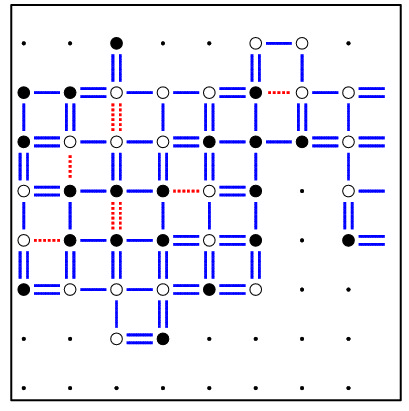
\includegraphics[scale =0.6]{img/edwards.jpg}
\caption{A representation of a 2D Edwards Anderson spin glass}
\label{fig:EA}
\end{figure}

 The EA model has been studied both with bimodal link distribution and Gaussian distribution. In fact, restricting on these two link distributions is typical in the spin glass problem. We recall that the bimodal link distribution is the one where each $J_{ij}$ is chosen from a set of two values (typically $\{\pm 1\}$), while the Gaussian link distribution is the one which has a probability density function for each link that is Gaussian. The major efforts of the analytical studies on EA model verted on the proprieties of the ground state of the system \cite{ground}.

It is important to underline that spin glasses are in general, and really in the majority of cases, very difficult if not impossible to solve exactly.

So far the number of widely accepted and tested solution to spin glass problems counts only one success. This is given by the mean field model.

\subsection{The mean field model}

The mean field model is a spin glass in which each couple of spin is interacting. The coupling constants probability distribution can be chosen as Gaussian, this time without loss of generality in virtue of the central limit theorem.

\begin{equation}
P(J) = \frac{1}{\sqrt{2 \pi {\delta J}^2}}\exp(-\frac{J-J_0}{2\delta^2})
\end{equation}

In order to maintain the Hamiltonian density $\mathcal{H}/N$ finite in the thermodynamic limit $\langle J^2\rangle-\langle J \rangle^2$ must be proportional to $1/N$.

This model has been proposed by Sherrington and Kirkpatrick \cite{SK}. Together with the definition, Sherrington and Kirkpatrick provided a valid solution for the high temperature phase \cite{SK2}. A general solution has been found years later by G. Parisi in 1985 \cite{beyond}.
In his solution, Parisi successfully evaluated the $q(x)$ order parameter using the replica method. Later his result has been demonstrated correct by further studies involving the cavity method \cite{guerra}.
Parisi showed for the first time that spin glasses have a complicated structure in the low temperature phase.

Let us outline in a few steps the most important passages of the Parisi solution and the difference with the SK solution. In \cite{SK2} the authors obtained a free energy functional that depends on the overlap values between each replica. By assuming that $q_{\alpha\beta}$ (where $\alpha$ and $\beta$ are replica indices) is equal for each couple of replicas, they developed a solution that is replica independent, simplifying much the final operations of the replica approach, that is the $n\rightarrow 0$ limit.
On the contrary Parisi assumed a $q_{\alpha\beta}$ different for each replica. He argued a particular structure for the $q_{\alpha\beta}$ (now called Parisi matrix).

A Parisi matrix is a block-hierarchical matrix. It consist of growing blocks placed along the diagonal, each block is itself a Parisi matrix of a smaller size. In order to generate an infinite number of different overlaps, Parisi imagined that before doing the $n\rightarrow 0$ limit, one must somehow do first the $n\rightarrow \infty$ limit.

\begin{figure}[h]
  \centering
  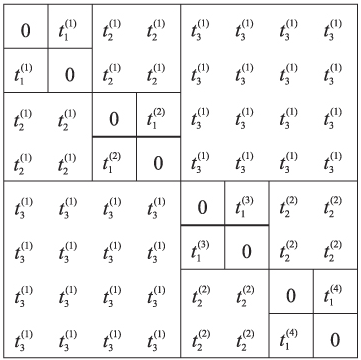
\includegraphics[scale =0.6]{img/matrix.png}\\
  \caption{Parisi matrix in a three step RSB}\label{}
\end{figure}

He then wrote the free energy functional as a function of three invariants of the Parisi matrix, that are
\begin{itemize}

\item{ $q_{\alpha\beta} q_{\beta\alpha} = \Tr q^2$}
\item{ $q_{\alpha\beta} q_{\beta\gamma} q_{\gamma\delta}q_{\delta\alpha} =  \Tr q^4$ }
\item{ $q_{\alpha\beta} q_{\beta\gamma} q_{\gamma\alpha}$ }

\end{itemize}

We remember that the third invariant is not $\Tr q^3$.
Using this particular choice of the matrix, Parisi has been able to evaluate these three invariants in an analytical way, arriving to a non trivial form for $q(x)$ in the $n\rightarrow 0 $ limit.

\section{A connection between two extremals}

The SK model turns out to be a good starting point for the investigation of more complicated models. Obtaining a solution for finite connectivity models (whose EA model is an excellent example) is indeed very complicated.

Let's now proceed in the definition of a somehow intermediate model. A sharp reader will note that the choice of the upcoming model is not casual. 

%\begin{quotation}

%- I'm searching the keys I've lost to get back home.\newline
%- Did you lost them here?\newline
%- No, honestly I do not have idea of where I lost'em..\newline
%- And why are you searching it here?\newline
%- Because, here, there is a light.\newline

%\end{quotation}

\newline
\begin{definition}

A Cayley tree with coordination number $K$ is an infinite connected cycle-free graph where each node is connected to $K+1$ neighbors.

\end{definition}


\begin{figure}[h]
\noindent
		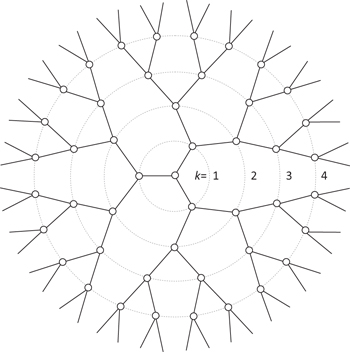
\includegraphics[scale =0.7]{img/cayley.jpg}
	\caption{Cayley tree with coordination number 2}
	\label{fig:cayley}
\end{figure}


Due to the limited number of neighbors, an exact solution of a spin glass defined on this lattice is not a mean field solution.
However in a Cayley tree there are no closed loops, and we will see later that this feature will allow us to derive a simple iterative scheme that will be used to obtain a solution.


\subsection{Boundaries of Cayley tree}

It is easy to check that the number of sites on the boundaries is a finite fraction even in the $N \rightarrow \infty$. The number of sites in the k-th shell $n_j$ can be written as a function of $n_{j-1}$.

\begin{eqnarray}
n_{j} &=& Kn_{j-1} \nonumber\\
      &=& K^2n_{j-2} \nonumber\\
		&=& ... \nonumber\\
		&=& K^{j-1}n_1 \nonumber\\
		&=& K^{j-1}(K+1) \nonumber\\
\end{eqnarray}

Thus the fraction of sites on the boundaries can be evaluated as

\begin{eqnarray}
\lim_{j\rightarrow\infty} \frac{n_{j}}{\sum_{j'=0}^{j-1} n_{j'}}
\end{eqnarray}

This fraction is evaluated in appendix A.
Since the number of boundary sites is relevant in the large N limit, it is preferable to
define our model in a subset of the Cayley tree.

\begin{definition}

A Bethe lattice of a Cayley tree with $L$ shells
is obtained considering only the first
$L'$ shells, where $L'/L \rightarrow 0$

\end{definition}

We empathize that Bethe lattice has no closed loops.

It is important to note that even with this definition, the effect of the
boundary sites is not negligible. In order to eliminate completely the
dependence of the model from the boundary conditions we define the Bethe lattice
as a random graph with fixed connectivity.

\begin{definition}

A random graph with fixed connectivity $K$ is a graph with exactly $K$ links for each node, with each link connecting two random nodes.

\end{definition}

A finite size random graph has closed
loops with length proportional to $\log N$, thus in the thermodynamic limit
the two models are locally equivalent. We will jump from the Bethe lattice to the random graph and viceversa,
depending on what is the most convenient to use in each particular tractation. As an example, when one performs a computer simulation the random graph turns out to be more convenient. However, when we will explain the analytical formulation of the solutions we will use the original Bethe lattice instead.

\begin{figure}[h]
\centering
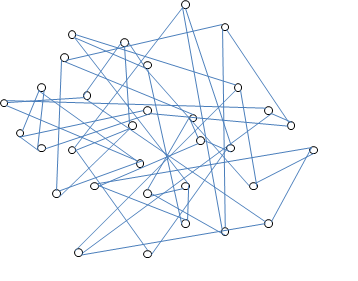
\includegraphics{img/randomgraph.png}
\caption{Random graph, in the large N limit equivalent to Bethe lattice}
\label{fig:}
\end{figure}

\section{Bethe lattice spin glass}

\subsection{Definition and Hamiltonian of the model}

Let's consider a set of $N$ Ising spins located on the sites of a Bethe lattice of coordination number $K$ . Each interaction (pictorially represented by each link in the lattice) is chosen at random between two values $\pm J$. $J$ will be set equal to 1. The Hamiltonian of the system is

\begin{equation}	
\mathcal{H}= \sum_{\<ij\>} J_{ij} \sigma_{i}\sigma{j}
\label{hamiltonian}
\end{equation}

where the symbol $\<ij\>$ indicates every couple $(i,j)$ connected by a link.

The main feature of this model is the tree-like structure of the lattice where it is defined. A tree is a graph where each pair of nodes (the sites) is connected by exactly a single simple path (the links).

Since the model is defined on a tree, each time we remove a site from the system, we divide it in $K$ subsystems, each non interacting with the others. Each subsystem has exactly the same structure of the lattice from which we removed a site. We will see in the next section that the action of these subsystems on the site removed (that now we re-insert) will lead to a self consistent equation relatively simple to understand.
We notice en-passant that this procedure will be possible due to the autosimilar structure of the Bethe lattice (more precisely, of the Cayley tree).

\section{Monte Carlo simulation of the spin glass}

During the early phase of this work, a Monte Carlo (MC) simulation of the system described has been performed. The algorithm used is a simple single spin flip with Metropolis acceptance (\cite{MCMC} for further readings on MCMC methods and Metropolis).
All the simulation have been made at temperature $T = 0.8$ with $K = 6 $; $T$ and $K$ have been chosen in order to compare my result with the one found in \ref{bethe} and \ref{zullo}.

\subsection{Generation of the random lattice}

The random lattice has been generated with an unusual procedure.
Let's remember what are the characteristics of a genuine random graph:
\begin{itemize}

\item{No auto links are present}
\item{Two sites must be connected by at most one link}
\item{Graph must not be divided in two or more non comunicating sub graph}

\end{itemize}

I have realize a random lattice using a simulated annealing. The cost function of the annealing is equal to the number of auto links plus the number of double links.
With this construction turns out that the cost of a good random graph is zero. The configurations are explored swapping the second extremals of two links taken at random. The configuration space with this evolution from a configuration to another is intuitively ergodic, and it is possible to create a genuine random graph in a someway small computation time.

Each time a genuine random graph is found by the annealing, a routine controls if the graph is bipartite; if not each link is saved into a new file and the routine is restarted with a different number of sites.
In this way I've generated a huge number of lattices, that later have been used in simulations.

\subsection{Evaluation of observables in a spin glass phase}

Since the MC evolution of the spin glass on Bethe lattice under the critical temperature is non ergodic, a single simulation risks to estimate badly the relevant observables, (I recall that it is possible to evaluate easily the mean magnetization, EA order parameter and internal energy in an easy way). Thus I've generated several copies of the system, some of them at temperature $T$, others at higher temperatures. The evolution of the system has been made with parallel tempering (for reference on parallel tempering \cite{tempering}), that allowed me to measure internal energy with relatively high precision.

\begin{equation}
U = -1.798 \pm 0.005
\end{equation}

In the past years researchers performed simulations on BLSG (as previously mentioned). An example is given by the simulations performed in Rome, reported in this article: \cite{zullo}. The authors evaluated the internal energy in the spin glass phase ($T = 0.8$) and obtained a value for $U$ of:
\begin{equation}
U = -1.799 \pm 0.001
\end{equation}


\part{Up to one RSB}

\chapter{The Bethe-Peierls solution}

The Bethe-Peierls solution was the first attempt to solve the BLSG model. Using the fact that the factorization approximation is exact on tree-like structures, the solution finds a self consistent equation for the field distribution $Q(h)$. However, we will se that the BP solution is not valid in the region of the glassy phase (under the critical temperature).In the low temperature phase we have to perform a much more refined computation (and we will do it in the following chapter).
In the next part of this chapter, the BP solution will be also referred as the replica symmetric (RS) solution. In fact, we will prove in the last section that the BP solution is equivalent to a replica symmetric solution in the replica framework \cite{bethe}.
A good description of the Bethe Peierls approximation in more general terms is available at \cite{montanari}.
The states structure at zero temperature, the phase transitions diagram and an algorithm generated for finding the ground states are discussed in \cite{tersenghi}.

Using the fact that no closed loops are present it is possible to solve
the problem by iteration \cite{hans}.
Our first task will be to write the partition function on a given site $\sigma_0$, which can be written formally as
a function of the local fields acting on $\sigma_0$

\begin{equation}
Z = \sum_{\sigma_0,\sigma_1,\ldot,\sigma_k} \exp{\beta( \sigma_0 \sum_{i=1}^{K} J_i \sigma_i + \sum_{i=1}^{K}h_i \sigma_i )}
\label{partition}
\end{equation}

Using the fact that $\sigma_0$ can only take values ${\pm1}$ it is possible to write each term of the partition function explicitly summing over $\sigma_0$

\begin{equation}
\sum_{ \sigma} \exp{ \beta ( \sigma_0 J \sigma + h \sigma)} = c(J,h)\exp{\beta u(J,h) \sigma_0}
\label{u}
\end{equation}

Where the two auxiliary function are defined as

\begin{equation}
u(J,h) = T \tanh^{-1}[\tanh(\beta J)\tanh(\beta h)]
\end{equation}

\begin{equation}
c(J,h) = 2 \frac{\cosh(\beta J)\cosh(\beta h)}{\cosh(\beta u(J,h))}
\end{equation}

We will see that the function $u(J,h)$ will return often in this discussion.
If we look the new form of equation \ref{u} we can see that in the new framework the effective Hamiltonian acting on $\sigma_0$ is the sum of the variables $u_1,\dots,u_K$ of each neighbor. We will call local field each $h_j$ interacting with a considered site.

If we sum the contribution from each branch, we can write
the magnetization on $\sigma_0$

\begin{equation}
\langle\sigma_0\rangle = \tanh(\beta h_0)
\label{sigma0}
\end{equation}

where $h_0$ is simply given by the sum of each effective field acting on $\sigma_0$.

\begin{equation}
h_0 = \sum_{i=1}^K u(J_i,h_i)
\label{merge}
\end{equation}

\begin{figure}
	\centering
		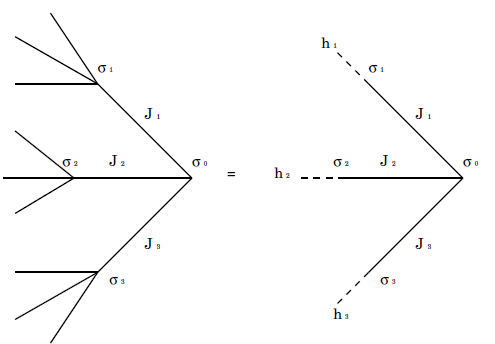
\includegraphics{img/tree.png}
	\caption{Pictorial representation of local fields on their branches}
	\label{fig:tree}
\end{figure}



\section{Cavity method for the Bethe lattice}

Before going on it is useful to recall the basic operations that will be used frequently in the elaboration. The formalism used in the next sections is usually referred as cavity method (\cite{beyond} for some generalities on the cavity approach). Since a large number of papers has been written on cavity method, here I will only remark the main tool we are going to use most frequently, that is the iteration procedure. We will show the method applied to the Cayley tree, since our utilization of it is directly aimed at a solution of the Bethe lattice spin glass.
Suppose to remove a random site from a Cayley tree(among with each of the links connected to it), now the system is divided into a number of subsystems equal to the coordination number $K+1$. Each subsystem is locally identical to the starting one.
Now suppose to have $K$ of these subsystems; if we pick up the root of each of those and merge into the site 0, we obtain an object that can be used to be merged to generate a bigger system, where now the site 0 is the root of one of the $K$ branches.

\begin{figure}[h]
\centering
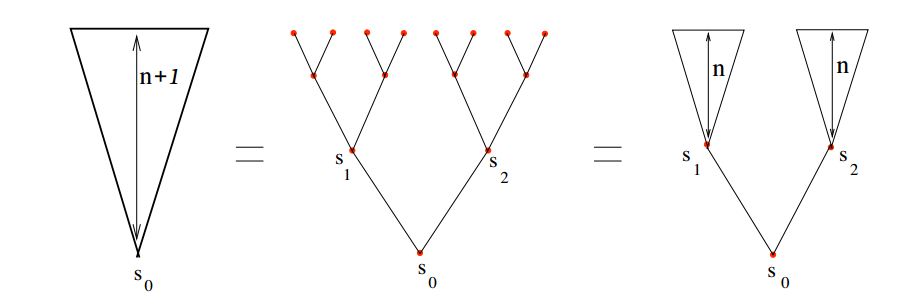
\includegraphics[scale =0.6]{img/cavity.png}
\caption{Scheme of the iteration procedure}
\label{fig:cav}
\end{figure}

This framework gives a method to obtain a recursion relation useful to solve the problem (that will be derived in the next lines) and an operative way to evaluate the relevant thermodynamic observables.
By imposing that each $u_j$ is derived from the same probability distribution $Q(h_j)$ of the site 0 we obtain a self consistent equation for $Q(h)$

\begin{equation}
Q(h) = \int dh_1Q(h_1),\ldots,dh_KQ(h_K) \delta(h-h_0)
\label{RS}
\end{equation}

In order to find the distribution of equilibrium local fields , given the distribution on a branch, we have to do the same operations as before, but now merging $K+1$ branches into one site. In this way we are adding a site fully connected to his neighbors, which cannot be used for an iterative costruction of the Bethe lattice, but will be used to find the site dependence of any relevant observable. When we add a site connected to $K+1$ branches we have

\begin{equation}
Q_t(H) = \int dh_1Q(h_1),\ldots,dh_KQ(h_K+1) \delta(h-H_0)
\label{true}
\end{equation}

\begin{figure}[h]
\centering
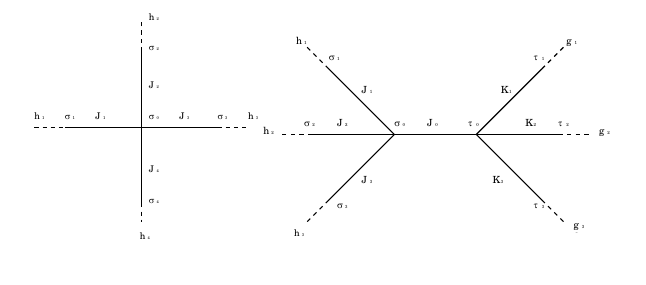
\includegraphics[scale =0.8]{img/sitebond.png}
\caption{Site and link contributions, in this figure the bonds linking the $\tau$ spin are labeled as $K_i$ (not to be confused with the coordination number K).}
\label{fig:sitebond}
\end{figure}

The field $H_0$ is calculated similarly to eq. \ref{merge} but this time using $K+1$ branches.

It is also possible to add a new link to the system, this time using a cavity link and, as a consequence, two cavity spins. Let's call these two spins $\sigma$ and $\tau$. These spins will be connected to $K$ neighbors, and when we add the new link $J_c$, they will be each other's $K+1$th neighbor.

Adding a link allows us to obtain the energy of the model (we remember that the energy $E$ is given by $E = \langle \mathcal{H} \rangle$). Since the Hamiltonian of the model is given by \ref{hamiltionian} the energy of the new link is simply given by

\begin{equation}
E_{c} = - J_c \langle \sigma \tau \rangle_c
\label{ec}
\end{equation}

where the average has a Gibbs measure with an effective Hamiltonian $\mathcal{H}_c$ which is given by

\begin{equation}
\mathcal{H}_c = - J_c \sigma \tau + h_0(\sigma)\sigma + h_0(\tau)\tau
\label{hc}
\end{equation}

where $h_0(\sigma)$ is the local field acting on $\sigma$ (given by $\tau$) before the insertion of the cavity link.
Using equation \ref{hc} in equation \ref{ec} allows us to find $E_c$: a simple computation gives a value for $E_c$ given by

 \begin{equation}
{E}_c = - J_c \frac{\tanh(\beta J_c)+\tanh(\beta h_0(\sigma))\tanh(\beta h_0(\tau))}
{1+\tanh(\beta J_c)\tanh(\beta h_0(\sigma))\tanh(\beta h_0(\tau))}
\label{links}
\end{equation}

\section{Overlaps and free energy evaluation}

The first observable we are going to evaluate, as a simple example, is the Edwards Anderson order parameter,$q ={1\over N} \sum_i \langle\sigma_i\rangle^2$.
Using \ref{sigma0} we can write $q$ as a weighted sum over the values of $H$

\begin{equation}
q = \int dHQ(H) \tanh(\beta H)\tanh(\beta H)
\label{qsite}
\end{equation}

It is also possible to compute the link overlap, which can be deduced from the iterative fields distribution, $Q(h)$ as ($E_J$ is the average over the $J$ distribution):

\begin{equation}
q_l = E_J \int dh_1Q(h_1)dh_2Q(h_2) \frac{\tanh(\beta J)+\tanh(\beta h_1)\tanh(\beta h_2)}
{1+\tanh(\beta J)\tanh(\beta h_1)\tanh(\beta h_2)}
\label{qlink}
\end{equation}


The free energy in this solution is evaluated as follows (for improved references one may see \cite{bethe} and \cite{katsu}):
First one must evaluate the site contribution to the free energy on the site $i$, then sum over the values of $\sigma_i$.

\begin{equation}
\beta {F_s}_i = \ln \sum_{\sigma_i} \exp(-\beta H_i \sigma_i )
\label{siteF}
\end{equation}

The link contribution is slightly more involved, as we need to add a cavity link, together with two cavity spins.
After a little computation and using equation \ref{links} is possible to write the link contribution to the free energy (\cite{bethe})

\begin{equation}
\beta {F_l}_ij = \ln \sum_{\sigma_i} \exp(-\beta H_iH_j \sigma_i\sigma_j )
\label{linkF}
\end{equation}

When both contributions have been obtained, it becomes possible to write the total free energy as the sum of the two contributions.
\begin{equation}
F = {K+1 \over 2}\sum_i F_l -KF_s
\label{RSF}
\end{equation}



\section{Computer implementation of the solution}

In order to control the correctness of the just proposed solution, it is possible to implement the solution just described using a population dynamics algorithm. This method has previously
been used in \cite{bethe} for the BLSG, and in \cite{self}

The algorithm is composed of a few little steps.

\begin{enumerate}
    \item{Generate $N_h$ fields. Fields may be i.i.d. random variables in the unitary interval, as example.}
    \item{Choose $K$ sites at random, among with $K$ values for $J$.}
    \item{Generate the field $h_0$ using \ref{merge}.}
    \item{Choose a site $i$ to update, this can be either random chosen or sequentially chosen.}
    \item{Substitute $h_i$ with $h_0$. Start again from point 2.}
\end{enumerate}

In this way one generates a Markov process in the fields distributions.
After a sufficient number of iterations is performed, the fields distribution will converge to the equilibrium one. We will see that, due to the presence of RSB in the low temperature phase (which has as a consequence a non ergodic behaviour of the system) this convergence is not assured, and the algorithm will need some improvements.

While this procedure generates the correct field distribution, it shall not be used to evaluate the site and field observables. In order to evaluate the overlaps, the internal energy and the free energy, we have to do the same operation as before, this time adding a new site to the system and a new link. Thus we have to merge $K+1$ branches into a new site for the site contributions, and we have to insert two new spins attached to $K$ branches each, and then merge those two, in order to get the correct link distribution. Once obtained these two one can evaluate every observable using equations \ref{qsite}, \ref{qlink}, \ref{siteF} and \ref{linkF}.

\subsection{Where the solution works}

If we solve numerically eq.\ref{RS} we note that, at least in the high temperature regime, we  have a paramagnetic solution. Surely if we put $Q(h) = \delta(h)$  \ref{RS} is satisfied. The solution is thus stable at high enough temperatures.
This was easily predictable: at high enough temperatures it is well known that finite connectivity spin glasses behave as paramagnets.

If we look at a numerical solution of equation \ref{RS} we may note that in the low temperature phase the $\delta$ solution becomes unstable. Past studies have shown that an evaluation of specific heat and entropy leads to a negative value for inverse temperatures $\beta>\beta_c$, where $\beta_c$ is given by the relation
\begin{equation}
\< \tanh( \beta_c J )\>_J = 1/K
\end{equation}



The instability of this solution has been widely investigated \cite{instability},\cite{thou},  \cite{tersenghi}. If considering the lattice used in my simulations and in \cite{zullo}, $K = 6$ and the inverse critical temperature is near 2.3.
The authors of \cite{zullo} performed simulation at temperature $T=0.8$, widely under the critical temperature.
In order to compare the results of the RS algorithm with the ones found in literature, the algorithm will run with $K=6$ and $T=0.8$.
The values returned by RS algorithm are reported in the following:

\begin{equation}
F = -1.863 \pm 0.001 \hspace{1 cm},U = -1.816 \pm 0.001 \hspace{1 cm}, q_0 = 0.683 \pm 0.001
\end{equation}

As we can see, the value of the internal energy $U$ totally disagrees with the one found in simulations.

\begin{figure}
\centering
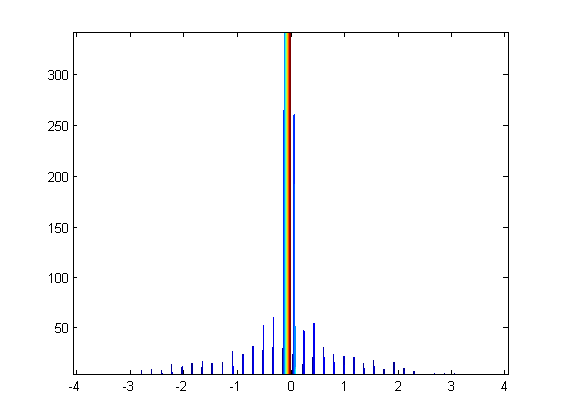
\includegraphics[scale 0.7]{img/fieldvsbeta.png}
\caption{The low temperature distributions (in blue) are not a \delta(h)}
\label{fig:}
\end{figure}


\section{Replica approach to the problem}

We ofter referred to the Bethe Peierls calling it the replica symmetric solution. In fact it is possible to prove the equivalence between the Bethe Peierls solution and a replica symmetric approximated solution in the replica framework. Details on the replica approach to spin glasses are available in all the major literature (examples are \cite{beyond} \cite{glass}). A computation of the free energy $F$ with the replica approach has been performed in \cite{replica}. In this paragraph we will only show that the replica symmetric free energy is equal to the one found in eq.\ref{RSF}.

In the replica framework the partition function \ref{partition} is replicated $n$ times. This means that now $\sigma$ in a n-dimensional vector of Ising variables. In order to reproduce the correct result, $n$ must go to zero at the end of the computations. In \ref{partition} the authors introduce a replica probability distribution, $\rho(\sigma)$ and the free energy functional $ F_r[\rho(\sigma)]$ with a structure similar to the variational free energy proposed in \ref{bethe}.
Let us report only the final result of the computation. Calling $f_r$ the free energy density $ F_r[\rho(\sigma)]/N$ we have

\begin{equation}
-\beta n f_r = {k+1\over2}\ln(\Tr_{\sigma,\tau} \rho(\sigma)^K\rho(\tau)^K \exp\sum_i \beta J \sigma_i \tau_i) -
k \ln Tr_\sigma \rho(\sigma)^{K+1})
\end{equation}

Let us comment this equation. As we can see, the free energy density is composed of two terms. The first is the same link contribution obtained in the previous section, while the other is exactly the site contribution. The link contribution has a K-th power because while we connect two cavity spins, each of those must be connected to $K$ sites, in order to maintain the fixed connectivity. On the contrary, the site contribution contains a power $K+1$.

If we set ${\delta F \over \delta \rho} = 0$ we obtain then correct replica free energy.

\section{Free energy shift}

It is possible to compute the mean free energy in the cavity approach, computing the free energy shift $\Delta F$ obtained by adding a new site or a new link to the system. The reason behind this equivalence can be explained as follows \cite{enzo}: when the equilibrium phase is reached, the total free energy may be written as $F_N = fN$; when adding a new spin we can simply write $F_{N+1} = f(N+1)$ and thus obtain the free energy per site by simply having $f = F_{N+1} - F_N \equiv \Delta F$.

Let's start by computing the site contribution to the free energy shift, $\Delta F_s $. Using the equation \ref{partition} and knowing that $\mathcal{Z} = \exp{-\beta F)$ we may write (\cite{bethe})
\begin{equation}
\beta \Delta F_s = \ln[2\cosh(\beta\sum_{i}^{K+1} u(J_i,h_i))] + \sum_{i}^{K+1} \ln[{\cosh\beta J_i \over \cosh \beta  u(J_i,h_i)}]
\label{sitedf}
\end{equation}

The bond contribution is more complicated, since it must be averaged over the $\sigma$ $\tau$ distribution.
\begin{eqnarray}
\beta \Delta F_l &=& \sum_{i}^K+1 \ln { \cosh (\beta J_i) \cosh (\beta L_i) \over  \cosh(beta u(J_i,h_i))\cosh(beta u(L_i,g_i))} \nonumber \\
&+&\ln[ \sum_{\sigma,\tau}\exp( \beta J \sigma \tau + \beta\sigma \sum_i^K u(J_i,h_i) \beta\tau\sum_i^K u(L_i,g_i) ) ] \nonumber \\
\label{linkdf}
\end{eqnarray}
In the above equation the variables $g_i$ represent the local fields acting on $\tau$, and $L_i$ are the bonds between each site.
The mean free energy is then evaluated as the sum of each site and bond contribution:
\begin{equation}
F = {(K+1)\over 2}\delta F_l - K \delta F_s
\end{equation}

It is also useful to report the iterative free energy shift, that is the free energy shift obtained when adding a site in the iterative construction of the Bethe lattice. It is simply given by the site contribution just evaluated, this time merging $K$ branches instead of $K+1$:
\begin{equation}
\beta \Delta F_{iter} = \ln[2\cosh(\beta\sum_{i}^K u(J_i,h_i))] + \sum_{i}^K \ln[{\cosh\beta J_i \over \cosh \beta  u(J_i,h_i)}]
\label{iterdf}
\end{equation}
This free energy shift will turn useful in the next chapter, when we will compute the probability distribution $Q(h)$ in the one step RSB framework. 
\chapter{Formulation of 1 step solution}

In this chapter I will present a solution (ideated by Mezard and Parisi, proposed in detail in \cite{bethe}) valid at a one step level of replica symmetry breaking, using the cavity method. Similarly to what has been done in the previous chapter, I will first derive the self consistent equation for the distribution of local fields, then I will show the equivalence with the replica formalism at a level of 1 RSB (that's why this solution will be called, despite the term may sound improper, 1 RSB solution). In the last section I will give a review of the results obtained by the authors of the original paper \cite{bethe}.

\section{Preliminary remarks}
If we introduce the possibility of the existence of many pure states the field probability distribution becomes different for every state. If we label each of these with $\alpha$ the probability distribution will depend on $\alpha$:

\begin{equation}
Q_i(\emph{h}) = \prod_\alpha Q_i(h^\alpha)
\end{equation}

The number of states $N_s$ must go to $+\infty$, but we can assume $N_s$ large but finite. Setting the value $N_s \rightarrow \infty$ too early may result in a bad definition of the field distribution.

The factorization over the states means that the probability distribution in each state is uncorrelated from the others. Simple cavity arguments can demonstrate that this assumption is correct for large $N_s$.

Every state has a probability distribution $\rho$ that follows an exponential law:

\begin{equation}
\rho(F) = \exp(-\beta x (F-F_R))
\label{distr}
\end{equation}

The reason of why the states are sampled with exponential distribution is found in the fact that \ref{distr} is the only distribution stable under little variations of $F$.

\begin{equation}
\rho(F+\delta F) = \exp(\beta x (F + \delta F-F_R))
\label{distrd}
\end{equation}

We will se now how the technique used to write the self consistent equation is similar to the one used in the replica symmetric solution, giving particuar emphasis on the step where replica symmetry is broken.

\subsection{Pure states and mixtures}

Since the term \emph{pure state} will be used often in the discussion, let us give briefly the definition of pure state. A state of a system is said to be a pure state if exists a measurable quantity that returns an outcome perfectly determined when evaluated on that state. A linear combination of pure states is a pure state.

\section{One step RSB with cavity method}

Let's start by considering again the BLSG. As in Bethe Peierls solution, we know that the field in the cavity site may be expressed in terms of the fields on the branches attached to it.

\begin{equation}
h_0^\alpha = \sum_{i=1}^K u(J_i,h_i^\alpha)
\label{merge1}
\end{equation}

Nevertheless a particular attention must be taken when we merge $K$ branches into our cavity site. When we add the cavity site to the system each of the previously uncorrelated branches becomes now correlated.
Let's call  $P_0(h_0,\Delta F)$ the joint distribution of $h_0$ and $\delta F$, of which the states $\alpha$ are a sample. When we merge $K$ branches the free energy $F^\alpha$ of each state will shift by $\delta F$: $G^\alpha =F^\alpha + \Delta F^\alpha$. The distribution of the new local field is given by

\begin{equation}
R_0(h_0,G) = C\int{dFd\[\Delta F\]\exp(\beta x(F-F^R))P_0(h_0,\Delta F)\delta(G - (F+\Delta F))}
\label{1RSB}
\end{equation}

It is convenient to write the joint distribution $R_0$ in terms of the field distribution.
\begin{equation}
R_0(h_0,G) = C'\exp(\beta x(G-F^R))Q_0(h_0)
\end{equation}

where $Q_0$ is the same field distribution of the RS solution, but weighted with the free energy shift, (here is the main difference with RS case, where this weight was not present in the integral self consistent equation; we will see later that each RSB step brings with him a reweigh at a different state level).

\begin{equation}
Q_0(h_0) = C\int{d[\Delta F]\exp(-\beta x\Delta F)P_0(h_0,\Delta F)}
\label{eqdf}
\end{equation}

If we take a close look to equation \label{1RSB} it is possible to give an interpretation of the terms it contains. The exponential weight gives the correct Boltzmann weight for the state considered, the joint distribution $P_0$ is the one containing information on the field distribution before the reweigh, the final delta is simply a selector of those free energies equal to  $F + \Delta F$.

It is now time to write the same recursion relation we wrote in the replica symmetric approximation. By having

\begin{equation}
Q_0(\emph{h})=Q(\emph{h})
\label{1solution}
\end{equation}
we obtain the recursion relation we were searching (we remember that the bold font is used to refer to the factorization on all states considered. In the end the number of states is sent to infinity. Note how the self consistent equation will change respect to the one found in \ref{RS}: in the simpler case we had only an uncorrelated distribution of $h$ and $\delta F$.
\begin{equation}
Q_0(h_0) = C\int{d[\Delta F]P_0(h_0,\Delta F)}
\end{equation}


\section{Evaluation of free energy}

Now that we take into account the co-existence of several pure states, every observable has to be averaged over the states distribution. Let's see how it is done, evaluating the iterative free energy and comparing it with the simple RS iterative free energy.

The site contribution of the free energy can be evaluated as follows ($E_J$ represents the average over all possible values of $J$, and is the averaging over the disorder):

\begin{equation}
-\beta F_s = E_J\langle \ln \sum_{\alpha} W^\alpha \exp[-\beta \Delta F_s(J_1\ldots,h_1\ldots,h_{K+1})] \rangle
\end{equation}

Using the theorem of Appendix C we can transform $F$ in a useful way

\begin{equation}
 F_s = -\frac{1}{\beta x} \langle \ln {1 \over N_s}\sum_{\alpha}\exp[-\beta \Delta F_s (J_1\ldots,h_1\ldots,h_{K+1})] \rangle
 \label{feval}
\end{equation}

The bond contribution is evaluated using the free energy shift obtained when adding a new cavity bond to the system (the variable $J$ without any index is the cavity bond:

\begin{equation}
-\beta F = E_JE_{L}\langle \ln \sum_{\alpha} W^\alpha \exp[-\beta \Delta F_l(J,J_1\ldots,h_1\ldots,L_1\ldots,g_1\ldots,g_{K},)] \rangle
\end{equation}


A simplified form  for $F$ is available evaluating two different site contributions, as previously happened in RS case.
In order to find the correct physical situation, it is well known \cite{wellknown} that one must find the value of the parameter $x$ for which the free energy $F$ is maximized. The x-derivative of equation \ref{feval},$d(x) = {dF \over dx}$ can be exactly evaluated.

\begin{equation}
d(x) = {-F\over x} - K d_s(x) + {K+1 \over 2} d_l(x)
\end{equation}

where the two contributions are given by

\begin{eqnarray}
d_s(x) &=& {-1\over \beta x} \log[ \sum_\alpha \exp(-\beta x \Delta {F_s}^\alpha) \log \Delta {F_s}^\alpha ]  \nonumber \\
d_l(x) &=& {-1\over \beta x} \log[ \sum_\alpha \exp(-\beta x \Delta {F_l}^\alpha) \log \Delta {F_s}^\alpha ] \nonumber
\end{eqnarray}

These two contributions will be derived in appendix B.
An evaluation of the zero of $d(x)$ returns a value of:

\begin{equation}
x* \equiv \{x:d(x)=0\} = 0.24 \pm 0.01
\label{star}
\end{equation}

If we compare the free energy formula with the one obtained in the replica symmetric approximation we may note that if we consider a single state $\alpha$ the free energy becomes equal to the free energy shift obtained in the previos sections.

\subsection{Equivalence with the replica formalism}

As in previous chapter, we redirect to a demonstration of the equivalence of the Mezard and Parisi solution with the replica solution at a level of one RSB.

In the one step RSB framework we have to divide the $n$ replicas into $n/x$ groups of replicas (labeled by \alpha).
\begin{equation}
\sigma_\alpha = \sum_{i \app \alpha} \sigma_i
\end{equation}

The authors of \cite{bethe} showed that, making an ansatz that restricts the possible probability distribution as factorized on the different block values, and using a result obtained in \cite{wong}, the one step RSB free energy is equivalent, in the small $n$ limit, to the one found in the preceding section.

We shall not provide the details of this procedure, which has been investigated in detail in \cite{bethe}.



\chapter{The one step RSB algorithm}

In this chapter I will give a brief description of the one step RSB algorithm, since the procedurenow  described is a part of the two step RSB one that will be developed in the next chapter. A full discussion may be found in \cite{bethe}. Since the method can be used

The algorithm is meant to implement equation \ref{1solution} using a population dynamics algorithm, in a similar way to what happens in the RS case. Obviously some modifications from the original algorithm are required.

The main difference relies in the presence of exponential weight in equation \ref{eqdf}

In order to reweigh the fields obtained according to \ref{eqdf}, we have to satisfy the following equation, \ref{reweigh}. We can see that equation \ref{reweigh} contains two cumulative distributions, the left member is the cumulative of the probability density function of the fields before the insertion of the cavity spin, while the right member is the one after this insertion.

\begin{equation}
\frac{1}{\sum_\alpha \exp(-\beta x \Delta F^{\alpha}) }\sum_\alpha \exp(-\beta x \Delta F^{\alpha}) \Theta(h-{h_{0}^{\alpha}}) = \frac{1}{N_s}\sum_\alpha \Theta(h-h^{\alpha})
\label{reweigh}
\end{equation}

There are various methods for obtaining this reweigh. Some have been investigated in \cite{bethe}. A general discussion is available on \cite{trattatello}. Once the correct fields are obtained, it is possible to evaluate every site and link observable, similary to what happened in the RS case. Every observable has to be averaged over the state distribution. We will see in the next section how this is performed.

Let's now summarize the passages of the one step RSB algorithm.

\begin{enumerate}
    \item{Define $N_h$ sites.}
    \item{For each site, generate $N_s$ fields. Fields may be i.i.d. random variables in the unitary interval, as example.}
    \item{Choose $K$ sites at random, among with $K$ values for $J$.}
    \item{For each field of each of the $K$ sites, generate the field $h_0$ using \ref{merge1}.}
    \item{The $N_s$ values for ${h_0}^\alpha$ (where $\alpha$ runs on $\{1,\ldots,N_s\}$) are not the fields that will be used in the merging population, at this point one has to consider the free energy shift given by equation \ref{eqdf}. This is done by generating a new population of fields $h^\alpha$ that, given the old set ${h_0}^\alpha$ satisfies equation \ref{reweigh}. }
    \item{Choose a site $i$ to update, this can be either random chosen or sequentially chosen.}
    \item{Substitute ${h_i}^\alpha$ with ${h_0}^\alpha$. Start again from point 3.}
\end{enumerate}

While this generates a field distribution that resembles the equilibrium one, it must not be used to compute the site and field observables. In order to evaluate the overlaps, the internal energy and the free energy, we have to do the same operation as before, this time adding a new site to the system and a new link. Thus we have to merge $K+1$ branches into a new site for the site contributions, and we have to insert two new spins attached to $K$ branches each, and then merge those two, in order to get the correct link distribution.

When we generate the true fields by merging $K+1$ branches we have to do the same procedure we do when we obtain the iterative fields $h_\alpha$, but using the site free energy $\Delta F_s$. In order to obtain the link quantities, such as the link contribution to the free energy, the internal energy and the link overlaps, we introduce the auxiliary field $v_0^\alpha$

\begin{equation}
v_0^{\alpha} = {1\over\beta}\atanh\frac{\tanh(\beta J) + \tanh(\beta h_0^{\alpha})\tanh(\beta g_0^{\alpha})}{1+\tanh(\beta J)\tanh(\beta  h_0^{\alpha})\tanh(\beta g_0^{\alpha})}
\end{equation}

The reweigh procedure for the $v_0^\alpha$ will be performed using the bond free energy shift $\Delta F_l$, evaluated using equation \ref{linkdf}.
Once the iterative fields, the site fields and the link auxiliary fields are obtained it is possible to evaluate every observable.

\subsection{Observables evaluation}

Using equation \ref{links} we can evaluate the internal energy $U$:

\begin{equation}
U= {1 \over N_s}\sum_{\alpha} \tanh (\beta v_\alpha)
\end{equation}

The overlaps are evaluated with the aid of equations \ref{qsite} and \ref{qlink}

\begin{eqnarray}
	q_0 &=& {1 \over N_s}\sum_{\alpha} \tanh(\beta h^{\alpha})\tanh(\beta h^{\alpha}) \nonumber  \\
	q_1 &=& {1 \over N_s} \sum_{\alpha'\neq\alpha} \tanh(\beta h^{\alpha})\tanh(\beta h^{\alpha'})\nonumber
\end{eqnarray}

The link overlaps are evaluated with the same set of equations, this time using $v^\alpha$ instead of $h_\alpha$.

\begin{eqnarray}
	q_0^{(l)} &=& {1 \over N_s}\sum_{\alpha} \tanh(\beta v^{\alpha})\tanh(\beta v^{\alpha})  \nonumber \\
	q_1^{(l)} &=& {1 \over N_s} \sum_{\alpha'\neq\alpha} \\tanh(\beta v^{\alpha})\tanh(\beta v^{\alpha'})\nonumber
\end{eqnarray}

The free energy is obtained summing the site and link contributions (equations \ref{sitedf} and \ref{linkdf}).

\begin{equation}
F = {K+1 \over 2} F_{l} - K F_s
\label{sitepluslink}
\end{equation}

It is also possible to compute the free energy using a different method. Since this does not involve a computation of the link observables and of the auxiliary fields $v_\alpha$, it has been used in the ealy phases of the investigation to obtain faster results in the free energy evaluation. On the saddle point the free energy may be evaluated using the iterative free energy $F_{iter}$ and the site free energy $F_s$. The total free energy can be estimated using the following formula \cite{bowman}

\begin{equation}
F = {K+1 \over 2} F_{iter} - {K-1 \over 2} F_s
\label{saddle}
\end{equation}

Moreover, differently from what happened in the RS case, we have to evaluate the site and bond contribution to the free energy x-derivative. These two contributions can be evaluated as:

\begin{eqnarray}
d_s(x) &=& {-1\over \beta x} \log[ \sum_\alpha \exp(-\beta x \Delta {F_s}^\alpha) \log \Delta {F_s}^\alpha ]  \nonumber \\
d_l(x) &=& {-1\over \beta x} \log[ \sum_\alpha \exp(-\beta x \Delta {F_l}^\alpha) \log \Delta {F_s}^\alpha ] \nonumber
\end{eqnarray}

\section{Comparison between RS and 1 RSB solutions}

It is useful to compare the results of \cite{bethe} to the ones obtained in the RS framework. In the RS theory we find the following values for the free energy $F$, internal energy $U$ and RS site overlap $q$

\begin{equation}
F = -1.863 \pm 0.002  \hspace{1 cm} ,U = -1.816 \pm 0.002  \hspace{1 cm} , q_0 = 0.6863 \pm 0.0002
\end{equation}

At a level of 1 RSB we have to find the value of $x$ that maximizes the free energy $F$. This has been estimated in \cite{bethe} and the authors found $x = 0.24$. The most relevant observables estimated with this value of $x$ are

\begin{eqnarray}
F &=& -1.858 \pm 0.002 , \hspace{1 cm}  U = -1.799 \pm 0.001 \nonumber \\
q_1 &=& 0.779 \pm 0.006 , \hspace{1 cm} q_0 =  0.30 \pm 0.02 \nonumber
\end{equation}

The results obtained in 1 RSB theory strongly improves the evaluation of $F$ and $U$.
We will show in the next section that is possible to improve further the results obtained. 



\part{Two step RSB}

\chapter{Two step RSB}

In this chapter I will investigate the two step RSB structure that is formally similar to the recursion relation found in the one RSB scheme. This will be executed by doing exactly the same steps as in one RSB solution, but this time using the one RSB solution itself as a starting point.

\section{From one to two steps}

I will divide each possible state $\alpha$ of the system into a large number of substates, each now labeled by $\gamma$ similarly to what we've done at a 1 step level. Let now $N_c$ be the number of states, and $N_s$ the number of substates, i.e. the number of states within a state.

It is possible to visualize this hierarchy pictorially using a tree-like structure.

\begin{figure}[t]
\centering
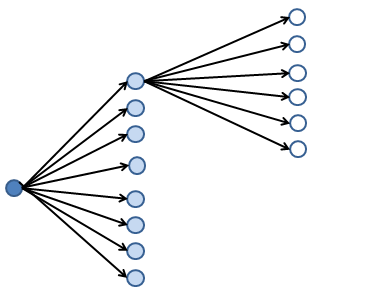
\includegraphics{img/twostep.png}
\caption{Two step RSB, states and substates are organized hierarchically}
\label{fig:2rsb}
\end{figure}

We assume now that each field distribution is independent from the one in other states or clusters.
In order to avoid confusion, the state level will be called \'Cluster level\', and the substate level will now be called
the \'state level\'.

\begin{equation}
Q_0(\emph{h})=\prod_\alpha Q(\emph{h}^\alpha)
\end{equation}

\begin{equation}
Q_0({\emph{h}^\alpha})=\prod_\gamma Q(h^{\alpha\gamma})
\end{equation}

Each state $\gamma$ has a proper weight that follows an exponential distribution. Similarly to what happens in one step RSB we can write
\begin{equation}
\rho(F^{\alpha\gamma}) = \exp(\beta x_s (F^{\alpha\gamma}-{F}^{\alpha}))
\label{distro2}
\end{equation}

Each cluster $\alpha$ has a proper weight that follows an exponential distribution too.
\begin{equation}
\rho(F^\alpha) = \exp(\beta x_C (F^\alpha-{F_R}))
\label{distro1}
\end{equation}

We will call $x_C$ the $x$ variable at a cluster level, in order to distinguish it from $x_s$, the $x$ variable at a state level. 
\section{Iterative construction}

The first step is the evaluation of every observable at state level: we have to generate the iterative fields $h_0^{\alpha\gamma}$, the site fields $H_0^{\alpha\gamma}$, obtained by adding a site to the system, and the link fields $v_0^{\alpha\gamma}$, the auxiliary fields obtained adding a link to the system (\cite{bethe} ). Every field is evaluated as follows:

\begin{equation}
h_0^{\alpha\gamma} = \mathcal{M}(h_1^{\alpha\gamma},\ldots,h_k^{\alpha\gamma})
\label{accazero}
\end{equation}
\begin{equation}
H_0^{\alpha\gamma} = \mathcal{M}(h_1^{\alpha\gamma},\ldots,h_{k+1}^{\alpha\gamma})
\end{equation}
\begin{equation}
v_0^{\alpha\gamma} = {1\over\beta}\atanh\frac{\tanh(\beta J) + \tanh(\beta h_0^{\alpha\gamma})\tanh(\beta g_0^{\alpha\gamma})}{1+\tanh(\beta J)\tanh(\beta  h_0^{\alpha\gamma})\tanh(\beta g_0^{\alpha\gamma})}
\end{equation}

where $g_0$ is evaluated using \ref{accazero}. These three fields are sampled at state level (the leaves of the tree). At each level we have to perform a reweigh with a weight given by equations \ref{distro2} and \label{distro1}. This will return the correct distribution that will we be used to perform the mean values that will be passed to the higher levels.
In order to evaluate each mean value we will take advantage of the equations reported in appendix C. 

Each time we add a step of RSB the only two operations we have to perform are a reweigh of its substates and a set of mean values calculations. This could suggest an iterative procedure to investigate the Bethe lattice spin glass at any desired level $l_{max}$ of RSB: 
The different weight at each level is moduled by the $x$ of the considered one. At each level $l$ we introduce a new parameter for $x$, and we have to determine which set of $\{x_1,\ldots ,x_{l_max} \in [0,1]^{l_max}$ maximizes $F$.

The only different level is the leaf one: at this stage we have to perform the merging procedure and find the values of $h_0$, $H_0$ and $v_0$. Once these are determined, we reweigh and average at each level $l$ using $x_l$.















\section{The algorithm}

In this section a procedure to create the field population is described, the detail of the algorithm will be reported in appendix A.
This algorithm implements the recursive reweigh at two levels.

We will call $N_h$ the number of fields of the systems, $N_s$ the number of substates in a given state, and $N_c$ the number of states (the states have been called clusters and the substates have been called states in the algorithm reported in the Appendix B).
Each field ${h_i}^{\alpha,\gamma}$ is initialized as iid random variables with uniform distribution.

Every iteration step we choose $k$ sites in $\{1,...,N_h\}$ that will be used for the merging procedure.

For each site $i_j$, $j=\{1,...,k\}$ we have $N_C$ clusters, each containing $N_s$ states. The merging procedure merges every same-state-same-cluster field taken from sites $i_1,...i_k$.
We will denote with $\mathcal{M}(\circ)$ the merging procedure. In order to evaluate the site and link quantities we need also to determine the true fields distribution and the auxiliary link fields distribution. Similarly to what has been done in the one RSB framework we can write

\begin{eqnarray}
h_0^{\alpha\gamma} &=& \mathcal{M}(h_{i_1}^{\alpha\gamma},\ldots,h_{i_K}^{\alpha\gamma}) \nonumber \\
H_0^{\alpha\gamma} &=& \mathcal{M}(h_{i_1'}^{\alpha\gamma},\ldots,h_{i_{K+1}'}^{\alpha\gamma}) \nonumber \\ g_0^{\alpha\gamma} &=& \mathcal{M}(h_{i_1''}^{\alpha\gamma},\ldots,h_{i_{K}''}^{\alpha\gamma}) \nonumber \\
v_0^{\alpha\gamma} &=& {1\over\beta}\atanh\frac{\tanh(\beta J) + \tanh(\beta h_0^{\alpha\gamma})\tanh(\beta g_0^{\alpha\gamma})}{1+\tanh(\beta J)\tanh(\beta  h_0^{\alpha\gamma})\tanh(\beta g_0^{\alpha\gamma})}\nonumber
\end{equation}

Once all the fields have been determined at a leaf level, it is possible to start the reweighing procedure at any level.
The first step is the reweighing at state level, done similarly as in one RSB. First thing to do is to evaluate the three free energies $\Delta F_{iter}$,$\Delta F_s$, $\Delta F_l$. This will be done with the aid of equations \ref{sitedf}, \ref{linkdf} and \ref{iterdf}.
The following step is the reweighing procedure, that must be done for each cluster, which means $N_c$ times per single step of population dynamic. This is realized by generating a set of new fields in order to satisfy the following equation

\begin{equation}
\frac{1}{\sum_\gamma \exp(-\beta x \delta F^{\alpha \gamma}) }\sum_\gamma \exp(-\beta x \delta F^{\alpha \gamma}) \Theta(h-{h_{0}^{\alpha\gamma}}) = \frac{1}{N_s}\sum_\gamma \Theta(h-h^{\alpha\gamma})
\label{reweighing}
\end{equation}

Once all the reweighs have been done at a state level, we can obtain the proper weight of each cluster simply evaluating the mean free energy shift $\langle dF\rangle_\alpha$ for that cluster. This can be done remembering how these are evaluated in the one RSB framework (equation \ref{feval})

Assigning a proper weight to each cluster allows us to reweigh at a two step RSB level. Similarly to what happens in the one-step RSB case, we may write
\begin{equation}
p_{\alpha} =\exp(-\beta x_C \langle dF\rangle_\alpha)
\end{equation}

The reweighing detail, both at state and cluster level, is reported in the Appendix. Once the clusters distribution has been reweighed, it is possible to evaluate the total free energy of the system, the overlaps and the other relevant observables.

\begin{figure}
		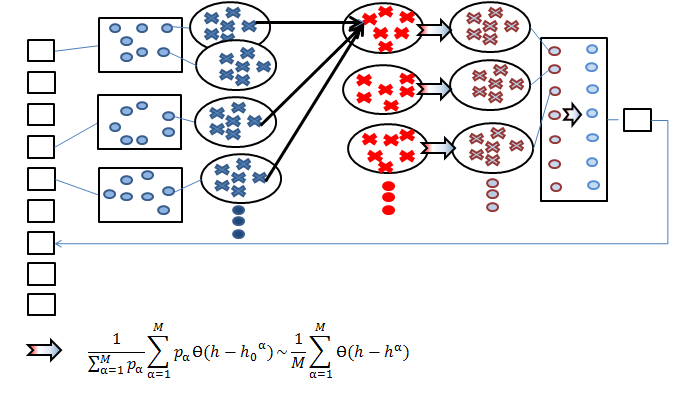
\includegraphics[scale = 0.7]{img/algoimg2.png}
	\caption{A step of the algorithm. In this figure the method used to generate the equilibrium fields is pictured: $K$ sites are chosen randomly. The states are merged according to \ref{merge} (represented with the black lines). Then the state distribution is reweighed in each cluster of the cavity site. Once all reweighs have been done at state level, the clusters are reweighed. The reweighing procedure is represented with the coloured arrow. Once all operations have been done, the new site replaces a site of the system.}
	\label{fig:algoimg}
\end{figure}

\subsection{Observables Evaluation}

Every observable is computed in a similar way to what happened in one step RSB section. There are two main differences from the one step RSB case.

\begin{itemize}

\item{Each observable has to be computed over every state and every cluster}
\item{There are two different derivatives, the $x_s$ derivative, and the $x_C$ one.}

\end{itemize}



\begin{equation}
U= -\sum_{\alpha\gamma} \tanh (\beta v_\alpha\gamma)
\end{equation}

The overlaps are evaluated with the aid of equations \ref{qsite} and \ref{qlink}, this time we have three overlaps, that can be computed in the following way.

\begin{eqnarray}
	q_2 &=& \sum_{\alpha\gamma} \tanh(\beta h^{\alpha\gamma})\tanh(\beta h^{\alpha\gamma}) \nonumber  \\
	q_1 &=&  \sum_{\gamma'\neq\gamma} \tanh(\beta h^{\alpha\gamma'})\tanh(\beta h^{\alpha\gamma})\nonumber \\
    q_0 &=&  \sum_{\alpha'\neq\alpha \gamma'\neq\gamma} \tanh(\beta h^{\alpha'\gamma'})\tanh(\beta h^{\alpha\gamma})\nonumber
\end{eqnarray}

The link overlaps are evaluated with the same set of equations, this time using $v^\alpha$ instead of $h_\alpha$. Again,. we have now to compute three different overlaps

\begin{eqnarray}
	q_2^{(l)} &=& \sum_{\alpha} \tanh(\beta v^{\alpha})\tanh(\beta v^{\alpha})  \nonumber \\
	q_1^{(l)} &=&  \sum_{\gamma'\neq\gamma} \tanh(\beta v^{\alpha\gamma'})\tanh(\beta v^{\alpha\gamma})\nonumber \\
    q_0^{(l)} &=&  \sum_{\alpha'\neq\alpha \gamma'\neq\gamma} \tanh(\beta v^{\alpha'\gamma'})\tanh(\beta v^{\alpha\gamma})\nonumber
\end{eqnarray}

The free energy is obtained summing the site and link contributions (equations \ref{sitedf} and \ref{linkdf}).

\begin{equation}
F = {K+1 \over 2} F_{l} - K F_s
\label{sitepluslink}
\end{equation}

As before, it is also possible to compute the free energy using a different method.

\begin{equation}
F = {K+1 \over 2} F_{iter} - {K-1 \over 2} F_s
\label{saddle}
\end{equation}

The two contributions to the $x_s$-derivative of the free energy are evaluated as in one step RSB case.

\begin{eqnarray}
d_s_{x_s}(x_s,x_C) &=& {-1\over \beta x_s} \log[ \sum_\alpha \exp(-\beta x \Delta {F_s}^\alpha) \log \Delta {F_s}^\alpha ]  \nonumber \\
d_l{x_s}(x_s,x_C)  &=& {-1\over \beta x_s} \log[ \sum_\alpha \exp(-\beta x \Delta {F_l}^\alpha) \log \Delta {F_s}^\alpha ] \nonumber
\end{eqnarray}


\section{The reweighing detail}

The reweighing procedure must generate a population of states distributed in order to satisfy equation \ref{reweighing}.

\begin{equation}
\frac{1}{\sum_\gamma \exp(-\beta x \delta F^{\alpha \gamma}) }\sum_\gamma \exp(-\beta x \delta F^{\alpha \gamma}) \Theta(h-{h_{0}^{\alpha\gamma}}) = \frac{1}{N_s} \sum_\gamma \Theta(h-h^{\alpha\gamma})
\end{equation}

The above equations can be implemented in a computer routine using various methods. In the simpler case we only choose the new states into a set containing the old states,
but with a weight given by their prefactor. In order to extract the new fields with the correct weight, the only operation that must be done is to sum over the weights and find the cumulative function of the distribution, then extract a random number in the unitary interval and check to which state it is associated in the cumulative function of the states.
This is indeed a risky procedure, since every new field is extracted from a discrete set, the one containing the old fields. If the system size is too small the risk is to produce a sample composed of a single field or two. This would make evaluation of every observable obviously go wrong.

I will like to remark that this procedure is done $N_c$ times for each iteration step, and one time reweighing $N_s$ variables, so a low complexity in this phase is mandatory.

\subsection{A more refined reweighing}

In this subsection I would like to spend a few words on the possibility of improving the reweighing procedure used in the algorithm runs. The algorithm just described is very simple to understand conceptually, but unfortunately it suffers a big bias given by the fact that it reweighs choosing the new elements from the starting set of the old ones. This in the large $N$ limit will not be a problem, but if the number of available starting states is small there is a chance that the algorithm will return a series of trivial results in a finite time, having generated for example the same value for all the states after the reweighing. An improvement of the reweighing procedure, however, will risk to overweigh the computational effort of the routine. An important thing to remark is that when one has to reweigh at the state level it is simple to create such routine, but when reweighing at cluster level the operation that one must do are conceptually different.

Let's start with the state level reweigh. In this case we have a set $\mathcal(S)$ of fields that sample a probability distribution. First of all we may sort the elements of $\mathcal(S)$, then we choose an element of $\mathcal(S)$ with a probability distribution given by each weight, let's call it $h_i$, where $i$ indicizes the element after the sorting procedure. Then we extract the new field in the interval that has as extremals $h_{i+1}$ and $h_i-1$. If the site chosen is an extremal, we may use the bounding support $[-K,K]$.

This procedure has the advantage of reshuffling a bit the numerical values of the data. This would make the algorithm stable even with small samples.

When we try to extend this reweigh to the cluster level, we need to slightly modify it. Since the data that we must reweigh now is not a collection of points, but instead a collection of probability distributions, we first need a definition of distance that will be used as a comparator in the sorting procedure. A common choose \cite{kullback} is to use the Kullback Leibler divergence as a metric (though it is not a well defined metric, since it is not symmetric). We recall that the Kullback Leibler divergence between two distributions $P$ and $Q$ measures how much information is lost when $Q$ is used to approximate $P$ and is defined as
\begin{equation}
D(P,Q) = \sum_i \log({P_i \over Q_i})P_i
\end{equation}
An ordering procedure could take Q as a the uniform distribution (we are sorting using the entropy of each distribution now) and sort the element with this criterion. The following step is to generate the new distribution. This can be done in an intuitive way similarly to what has been done for the states.

The last passage is the reshuffling of the new fields in each cluster, and then the reshuffle for each cluster. This is mandatory because the ordering procedure introduces a bias, and the reshuffle sets again the correct situation. The reshuffle procedure is very fast (linear in the data size) and typically the Fisher Yates shuffle is used \cite{shuffle}.

\subsection{The effect of reweighing and the meaning of x}

Let's point out how the reweighing of the fields modifies the field distribution. In this section I would like to a couple of graphs representing how the fields will evolve without reweighing. If we try to evolve the fields set without reweighing (no matter how many states or how many clusters we have) we simply obtain the RS algorithm. 

As we can see using appendix C, a value of $x=0$ means that each weight except one is zero. Thus
only those those states associated with that weight are statistically relevant. Ths is equivalent to an assumption that no RSB is present at that level. As an opposite situation, a value for $x$ equal to one means that each state
has the same proper weight, sending the measure of each state to zero. As we can see, the level two $x$ variable, $x_C$, is not that far from zero. This shows a result anticipated before, two step RSB is present, but its
improvement from the one step solution is more subtle than the one obtained passing from RS to one step RSB. So the effect of the reweighing could be small at low values of $x$. In order to make
the distinction clear to the observer, I ran the algorithm once with a value of $x_C = 1$ and $x_s = 1$. The effect of the reweighing is pictured in figure \ref{reweighfig}.

\begin{figure}
  \centering
  % Requires \usepackage{graphicx}
  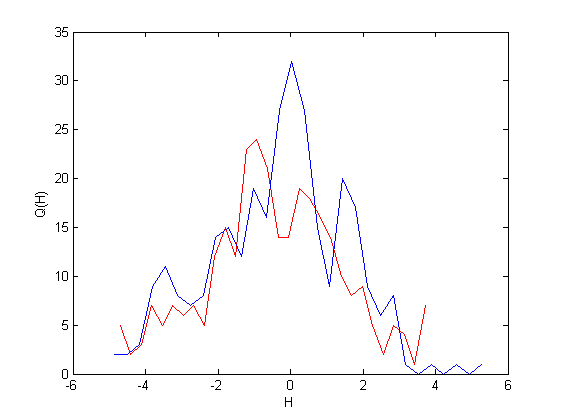
\includegraphics[scale = 0.7]{img/reweigh.pg}
  \caption{Reweighing of the fields $h_0^{\alpha_0 \gamma}$ in cluster $0$ at a state level with $x_C=1,x_s = 1$. In blue we have the fields distribution before the reweighing, in red the distribution after the reweigh.}\label{reweighfig}
\end{figure}










\chapter{Results}

In this chapter I am going to illustrate the results obtained when running the algorithm. This include an evaluation of the system free energy and site overlaps. It is possible to give a quantitative description of the correctness of the solution. This will be done in the final section, introducing a RSB sensitive parameter and comparing the result obtained in \cite{bethe}, the results obtained from \cite{zullo} and ours.

\section{Evaluation of $x_{C,max}$ and $x_{s,max}$}

In order to evaluate the thermodynamic procedures, it is well known that first of all one must maximize the free energy respect to $x_s$ and $x_C$.
We will call  $x_{C,max}$ and $x_{s,max}$ the two values that determine the maximum.
A direct computation of the free energy is possible using the corollaries in appendix III. Our task is to find a maximum of $F$ inside the range
$(x_s,x_C)\app \[(0,1) \times (0,1)\]$.

I made several runs of the algorithm, varying $x_s$ and $x_C$ and evaluating the mean free energy on many iterations.
Since a previous evaluation of one step RSB $x$ has been made \cite{bethe}, finding a value for $x_{max} = 0.24 $ and an incredibly accurate estimation of the free energy, we will expect to find the two values in a region close to the couple $(x_{max} , x_{max})$.




\section{Various run methods}

Since we have more than one task to accomplish, every run of the algorithm will differ a bit from the others, depending on which is the main goal of that particular run.
In order to explain better, let us summarize each run and its goal.

\begin{enumerate}
 \item{Find the region which maximizes $F$. This can be done with low precision, just to give a hint on where to concentrate in future.}
 \item{Perform high precision runs on the region found previously. The goal is to find the correct couple $X \equiv(x_C,x_s)$ with sufficient high precision.}
 \item{Perform a number of runs with different values of $N_c$, $N_s$ and $N_h$. This will allow us to extrapolate the thermodynamic limit using an interpolation.}
 \item{Once the couple $X$ has been found, we can perform a number of simulations with parameters $X$, in order to get each observable with relatively small error}
\end{enumerate}

A first computation has been made using low values for $N_h$, $N_c$ and $N_s$. This will give us a first hint on where to find the searched maximum.

\begin{figure}[h]
	\centering
		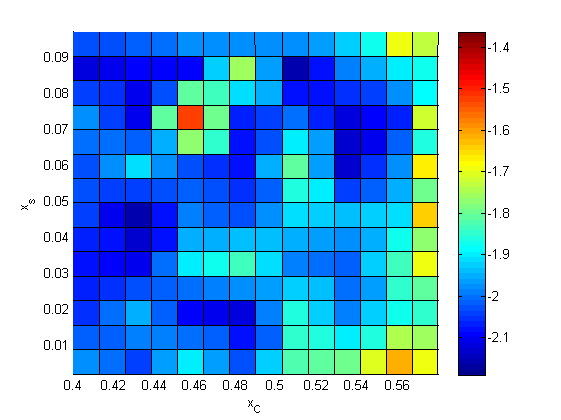
\includegraphics[scale=0.8]{img/generic_F.png}

		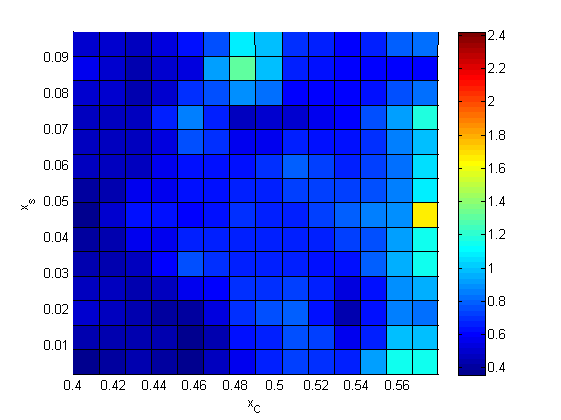
\includegraphics[scale=0.8]{img/generic_err.png}
\caption{Evaluation of F using brute force. 64 runs have been performed with low precision. }
\end{figure}

As we can see from figure, even if the free energy value is wrong we are now able to determine the correct region for our investigation.
Once the best region has been found, it is possible to enclose the search range in a neighborhood of these values.

\begin{figure}[h]
   \centering
		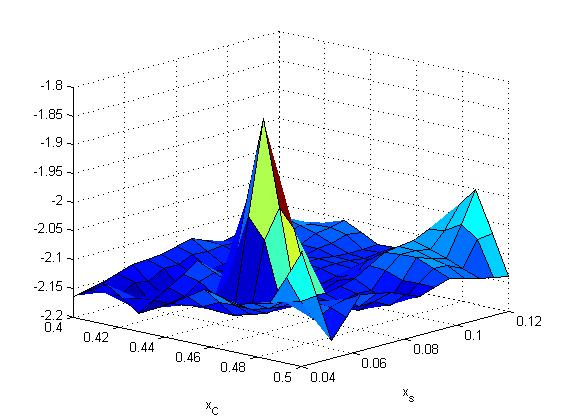
\includegraphics[scale = 0.6]{img/refined.jpg}
\caption{Evaluation of F in a smaller region}
\label{refined}
\end{figure}

From a finer computation we can see that the couple that maximizes the free energy is given by:

\begin{equation}
x_{s,max} = 0.07 \pm .01 \hspace x_{C,max} = 0.45 \pm .05
\end{equation}

Results obtained have an easy interpretation; in fact it is possible to make two interesting argumentations:

\begin{itemize}

\item{The value of both $x_C$ and $x_s$ is clearly nonzero, this
			means that replica symmetry is broken at a cluster level.
			It is now almost sure that the exact solution involves continuous RSB. Going to higher levels of RSB however would need a large computation effort.}

\item{The error in the determination of the maximum is much larger in the $x_C$ direction, evidencing the fact that the evaluation of two step RSB corrections need a greater computation effort to be
    evaluated.}
\end{itemize}

\newpage

\section{Analysis of finite-size error}

Now we evaluate the dependence of the observable averages returned by the algorithm from the sample size.
What we will do is to evaluate the average free energy of the system as a function of $N$, and then plot $F(N)$ versus $N^{-1}$. The $N\rightarrow\infty$ result is extrapolated from a polinomial fit on the obtained distribution
\begin{figure}
	\centering
		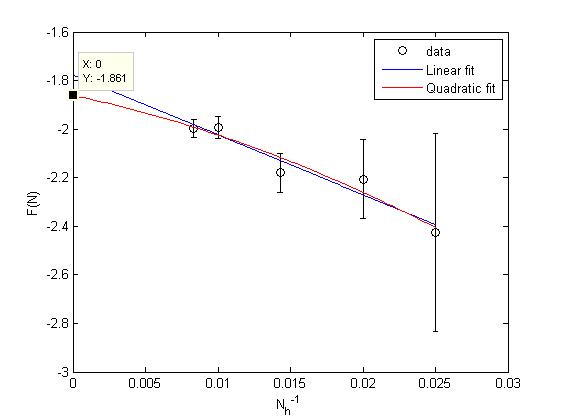
\includegraphics[scale = 0.6]{img/polyN.jpg}
		\caption{Polinomial fits of the efficiency of the results}
\end{figure}

The algorithm runs have been performed first on a domestic computer. We can see from the figure that the measurements are affected by large sistematic errors at low values of $N$. Using a domestic computer it was possible to reach values of $N$ not greater than 50.
In the figure shown above we can see that, due to limited computation capability, our algorithm cannot make a sufficienly accurate prevision in the thermodynamic region (large $N$).

It is expected that good results may be obtained with values of $N$ in the surroundings of 500. Since these numbers are out of the range of my personal computer, the simulations are currently in preparation for a run on a cluster calculator located in Sapienza University.

%We can compare the finite-size error of the two evaluation methods for the free energy $F$.
%We remark that we previously found two alternative methods for the free energy evaluation that were given by

%\begin{eqnarray}
%F &=& {K+1\over 2} F_l - K F_s \nonumber \\
%F &=& {K+1\over 2} F_{iter} - {K-1 \over 2} F_s \nonumber
%\end{eqnarray}


 %\begin{figure}
 %	\centering
 %		\includegraphics[scale = 0.6]{img/comparison.jpg}
 %		\caption{Polinomial fits of the efficiency of the results}
 %\end{figure}




\subsection{Another finite size problem}

Since the reweighing procedure only reshuffles the fields according to their free energy shifts (equation \ref{dfiter}), it is possible that, after a certain number of iterations, the population is sampled from a restricted set of clusters. By iterating again could rise the possibility of sampling the population from a single cluster. If we look equation \ref{dfiter} and try to compute $\Delta F$ using a populations where all clusters are the same, we may end having a problem in the free energy evaluation (depending on the particular type of error occurred the free energy evaluation could lead to a machine $0$ or a Nan). In order to avoid this possibility, I decided to add a
small perturbation to the evaluation of the $h_0 ^ {\alpha\gamma}$ fields. From physical argumentations \cite{vulpiani} one can deduce that the correct states distribution $Q(h)$ is left invariate under little perturbations of itself. This granted a sufficiently low reshuffling of each state distribution within each cluster. Obviously the insertion of a noise underestimates the overlaps



\section{Observables}

\subsection{Site Observables}

There are now three site overlaps that must be evaluated:
\begin{itemize}

\item{The self overlap, $q_2$, computed averaging over each state $\gamma$ and over each cluster $\alpha$}
\item{The same state overlap, $q_1$, computed averaging over each state $\gamma'$ different from $\gamma$}
\item{The interstate overlap, $q_0$, computed averaging over each cluster $\alpha'$ different from $\alpha$, and over each state $\gamma'$ different from $\gamma$}

\end{itemize}

\begin{eqnarray}
	q_2 = \sum_{\alpha, \gamma } \tanh(\beta h^{\alpha\gamma})\tanh(\beta h^{\alpha\gamma})  \\
	q_1 = \sum_{\alpha, \gamma} \sum_{\gamma' \neq \gamma } \tanh(\beta h^{\alpha\gamma})\tanh(\beta h^{\alpha\gamma'})  \\
	q_0 = \sum_{\alpha, \gamma} \sum_{\gamma' \neq \gamma, \alpha' \neq \alpha} \tanh(\beta h^{\alpha\gamma})\tanh(\beta h^{\alpha'\gamma'})  \\
\end{eqnarray}

Each of these values is then averaged over every site and every iteration.
A computation of these values near the critical point $X = (x_{s,max},x_{C,max})$ gives back these three values for the overlaps

\begin{eqnarray}
	q_2 = 0.71 \pm .005\nonumber \\
	q_1 = 0.31 \pm .03 \nonumber \\
	q_0 = 0.19 \pm .03 \nonumber \\
\end{eqnarray}

It is possible to give a quantitative evaluation of the correctness of the two-step RSB implementation. Let us define
\begin{equation}
R = \int q^4 P(q)dq - (\int q^2P(q)dq)^2
\label{erre}
\end{equation}

It is worth noting that in a RS theory $R=0$, while in \cite{bethe} the authors obtain $R = 0.047 \pm 0.002$. Simulations return a value for $R=0.056 \pm 0.001$, while the one obtained in the 2 step RSB framework can be evaluated as follows:
\begin{equation}
P(q) = p_0 \delta(q-q_0) + p_1 \delta(q-q_1) + p_2 \delta(q-q_2)
\end{equation}
where each $p_i$ is given by
\begin{eqnarray}
p_2 = (x_C) \nonumber \\
p_1 = (x_s - x_C) \nonumber \\
p_0 = (1 -  x_s)  \nonumber \\
\end{eqnarray}
A direct computation returns a value for $R =0.06$, with an high error associated:

\begin{equation}
                        R =0.06 \pm 0.02
\end{equation}

We may note that the error on the estimation of $R$ is very high. This is due to the imprecise location of $x_C$ at finite cluster size, together with a high variability of $R$ on small changes of the overlaps and the two values of the $X$ couple. Since R depends on five parameters, only a very accurate estimation of these will lead to a value

I would like to end this section with a plot of the $q(x)$ function, limited to the two step RSB framework. This has been painted using the three overlaps found previously

\begin{figure}
  \centering
  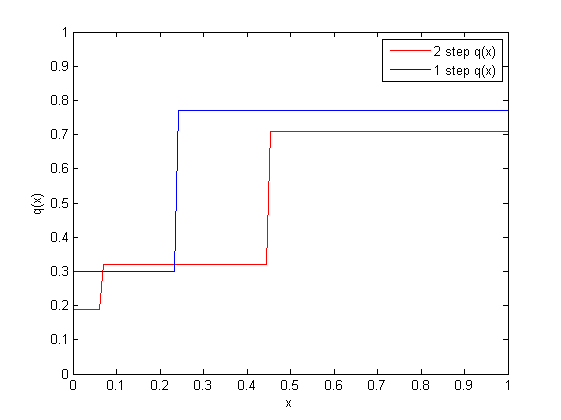
\includegraphics{img/q_function.png}
  \caption{Evaluation of R}
\end{figure}
\subsection{Link Observables}

First of all we report the evaluation of the link overlaps.

\begin{eqnarray}
	q_2^{l} = 0.73 \pm .01\nonumber \\
	q_1^{l} = 0.28 \pm .03 \nonumber \\
	q_0^{l} = 0.17 \pm .03 \nonumber \\
\end{eqnarray}

The next variable we want to compute is the internal energy of the system, given by equation

\begin{equation}
U = - \sum_{\alpha \gamma} \tanh{\beta v^{\alpha\gamma}
\end{equation}

A computation of $U$ returns a value in very good agreement with the simulations:


\begin{equation}
U = -  1.799 \pm 0.001
\end{equation}

This result needs a particular remark, since $U$ is the only observable easily computable in Monte Carlo simulations.
We may note that
Such a good agreement is very important for the validation of the procedure.

\section{Error evaluation}

In this section I will discuss on the error associated to the evaluation of each quantity.  For each algorithm run we obtain a set of values for $q_i$ (we will call them $q_i(t)$, with $i = {0,1,2}$ and $t=0,1,\ldots,T$. $T$ is sufficient large number), and  set of values for $F$, name it $F(t)$. Any formula valid for the three observable will be written using the variable $Y$, with $Y$ the quantity considered.

From these strings we main obtain the average value over one simulation $Y = {1\over T}\sum_t Y(t)$. If we evaluate the variance $\sigma_{sim}$on $Y$ using $Y(t)$ we obtain a value that has an intrinsic error due to the limited number of RSB steps. Since the three values are an approximation of a function $q(x)$, the error estimated will not go to zero in the large samples limit. A correct procedure in the error evaluation is to collect a large number of samples, one per each simulation, and evaluate the mean value and the variance over these sets. If we call $s$ the index that runs over the simulation number and $N_s$ the number of simulations performed with a particular set of $x_C$ and $x_s$, we can write
\begin{equation}
Y={1\over N_s} \sum_s {1\over T} \sum_t Y_s (t)
\end{equation}

The correct value for the variance can be estimated using the values obained from each simulation $Y_s = Y = {1\over T}\sum_t Y_s(t)$:
\begin{equation}
{\sigma^2}_Y={1\over N_s - 1} \sum_s (Y-Y_s)^2
\end{equation}

The same procedure can be applied in the computation of R, given by equation \ref{erre}

It is important to underline the fact that these values are affected by very big sistematic errors. As shown in the previous section, using the small values of $N$ for the runs performed will result in a very poor accuracy in the evaluation of the two step RSB observables.






\chapter{Conclusion of the work}

In this conclusive chapter I will regroup the results obtained. A small section will be dedicated to the possibility of extending the method described to higher levels of RSB.

The main task of this study was to give a quantitative evaluation of the two step RSB  relevant observables (with a particular attention to $q_0$, $q_1$ and $q_2$. It has been shown that results are compatible with two step broken symmetry. Similarly to what happens in the SK model, replica symmetry is broken in a complicated way.
It is possible to argue that RSB is present at any level. In line of principle the algorithm used can be extended to highers levels of RSB. Since it is possible to reach high levels of algorithmical complexity with modern cluster computer (I personally believe that a good result may be obtained up to four RSB levels, though the utility of such computation is not obvious), it would be interesting to develop a recursive version of the algorithm described in chapter 5, capable of reaching any desired level of RSB.

A possible future investigation can be done on a way to increase the algorithm's computational efficiency. This might be mandatory if one wants to reach higher levels of RSB. Since the algorithm's complexity, as described in this work, has a complexity equal to $N_h N_c {N_s} ^ 2$, a good estimation of the relevant observables is complicated even in this two step RSB case. However, although the low precision of the runs performed, the algorithm has been capable to achieve good enough results.

The results obtained may also give us a hint on the shape of the Parisi overlap function $q(x)$. As we can see from the values of $x_i$ (where $i$ for now can only be chosen between $\{ s, C\}$), these two tend to be more or less near to zero. This indicates a fast increasing $q(x)$ in the left region of the interval $x \app [0,1]$, similarly to a result obtained on other spin glass systems\cite{function}.


\backmatter \appendix

\chapter{Boundaries of the Cayley tree}

Consider a Cayley tree of coordination number $K$. The number of site on a given shell $s$ can be evaluated as follows:

\begin{eqnarray}
n_{s} &=& Kn_{s-1} \nonumber\\
      &=& K^2n_{s-2} \nonumber\\
		&=& ... \nonumber\\
		&=& K^{s-1}n_1 \nonumber\\
		&=& K^{s-1}(K+1)n_0 \nonumber\\
\end{eqnarray}

where $n_0=1$ and represents the seed of the lattice. The fraction of sites lying on the boundary is evaluated using

\begin{eqnarray}
\lim_{s\rightarrow\infty} \frac{n_{s}}{\sum_{j=0}^{s-1} n_{j}}
\end{eqnarray}

The sum on the denominator of the equation is easy to determine. If we regroup the $(K+1)$ common factor we may evaluate the sum as a truncated geometric series. It is well know that a sum of the type $\sum_{j=0}^n x^j$ can be estimated as $ {1-x^{n+1} \over 1 - x} $. Thus it is possible to write (remembering that each $n_j$ contains a term proportional to $K^j-1$ and the last term has $j=s-1$, and neglecting the first term of the series when extracting the common term $K+1$)

\begin{eqnarray}
\lim_{s\rightarrow\infty} \frac{n_{s}}{\sum_{j=0}^{s-1} n_{j}} &=&  {(K+1)K^{s-1}\over
{(K+1)(1-K^{s-1}) \over (K+1)}} \nonumber \\
                                                               &=&  {K^{s-1}(1-K)  \over 1-K^{s-1}} \nonumber \\
                                                               &=&   K \nonumber
\end{eqnarray}

Thus the for each site in the internal region of the Cayley tree we may find $K$ sites on the frontier, in the thermodynamic limit.

%\chapter{Evaluation of the x-derivative of the free energy}

%Before starting we remind that the total free energy of the BLSG may be written as $F = {K+1 \over 2}F_l - K F_s$, where
%$F_l$ and $F_s$ are respectively given by
%
%\begin{eqnarray}
%-\beta F_s &=& E_J\langle \ln \sum_{\alpha} W^\alpha \exp[-\beta \Delta F_s(J_1\ldots,h_1\ldots,h_{K+1})] \rangle \nonumber \\
%-\beta F_l &=& E_JE_{L}\langle \ln \sum_{\alpha} W^\alpha \exp[-\beta \Delta F_l(J,J_1\ldots,h_1\ldots,L_1\ldots,g_1\ldots,g_{K},)] \rangle \nonumber
%\end{eqnarray}%

%The bond contribution is evaluated using the free energy shift obtained when adding a new cavity
%bond to the system (the variable $J$ without any index is the cavity bond).
%If we perform the x-derivative of $F(x)$ we obtain
%


\chapter{Weighted sums with exponential density}

Here is a list of two theorems useful to evaluate weighted averages in the RSB scheme.

\begin{theorem}

Consider a set of $M$ iid random free energies, distributed with the exponential density $\rho(f) \propto \exp(\beta x (f-f_R))$. Then, neglecting terms which go to
zero when $M$ goes to infinity, the following relation holds:

\begin{equation}
\langle \ln \frac{ \sum_k a_k \exp(-\beta f_k) }{\sum_k \exp(-\beta f_k)}\rangle = \frac{1}{x} \ln (\frac{1}{M} \sum_k a_{k}^x)
\label{app1}
\end{equation}
\end{theorem}

\begin{corollary}
With the same conditions of the previous theorem, the following relation is valid.

\begin{equation}
\langle\frac{ \sum_k a_k b_k\exp(-\beta f_k) }{\sum_k a_k\exp(-\beta f_k)}\rangle = \frac{ \sum_k a_{k}^x b_k}{\sum_k a_{k}^x}
\label{app2}
\end{equation}
\end{corollary}

As it is easy to see, once \ref{app1} is demonstrated, \ref{app2} follows in a straightforward way.


\chapter{Algorithm core}
\section{Main part}
The main file of the two step RSB algorithm is reported. The main file performs a simulation for each pair of the values in the x_rsb_sample and y_rsb_sample arrays (called $x_s$ and $x_C$ in the discussion).

In the first phase of the study the goal was to find the couple that maximizes $F$, so the range of the couple $(x_s,x_C)$ was in this way easy to configure.
When the correct couple has been found, the same procedure shall be used to do estimate the error
in the evaluation of each observable.

\begin{verbatim}

#include "defines.h"

int main(){

	//be polite	
	cout << "hello!";


	//random seed for randStream
	srand(0);

	//remove previous data
	remove(FILE_NAME_XY);

	//initialize variables
	mySystem Sys;

	//init del sistema
	init();


	//////////////////////////////////////////////////////////////////////////////////////////
	//////////////////////////////////////////////////////////////////////////////////////////
	Sys.time = 0;
	while (Sys.time < MAX_TIME)
	{

		//choose indexes
		Sys.currSiteIndex = Sys.time%Nh;
		Sys.currSite = &Sys.Site[Sys.currSiteIndex];

		Sys.choose_sites();

		//merge
		Sys.merge_fields();

		//reweigh
		Sys.currSite->reweigh();

		//evaluate free energy
		Sys.currSite->evaluate();

		if (Sys.time > BIAS && Sys.time % Nh == 0){

			//observables
			Sys.evaluate_observables();
			Sys.write_file();
		}

		if (Sys.time == MAX_TIME / 2){
			cout << "Halfway done ";
		}
		if (Sys.time % (MAX_TIME / 10) == 0){
			cout << ".";
		}

		Sys.time++;

	}//endsim

	return 0;
}



\end{verbatim}

\section{Merge procedure and free energy shift}

In this appendix I will provide the routine used when merging $K$ branches into a site. In this code I will also evaluate the free energy shift, at state level.

\begin{verbatim}
void mySystem::merge_fields(){

	// evaluate for each cluster & state the
	// merged field and the free energy
	double u, usite, ulink;
	double beta = 1. / T;
	double shift,shiftsite,shiftlink1,shiftlink2;

	double h0,h0site,h0link,g0link;

	for (int cit = 0; cit < Nc; cit++){
		for (int sit = 0; sit < Nc; sit++)
		{
			h0 = 0;
			h0site = 0;
			h0link=0;
			g0link = 0;
			shift = 0;
			shiftsite = 0;
			shiftlink1 = 0;
			shiftlink2 = 0;
			for (int k = 0; k < 2 * K; k++){
				if (k < K){
					u = T*atanh(tanh(beta*Jiter[k])*
						tanh(beta*Site[iterNeighs[k]].Cluster[cit].State[sit]));
					h0 += u;
					shift += log(cosh(beta*Jiter[k]) / cosh(beta*u));
				}
				if (k < K + 1){
					usite = T*atanh(tanh(beta*Jsite[k])*
						tanh(beta*Site[siteNeighs[k]].Cluster[cit].State[sit]));
					shiftsite += log(cosh(beta*Jsite[k]) / cosh(beta*usite));
					h0site += usite;
				}
				if (k < K){
					ulink = T*atanh(tanh(beta*Jlink[k])*
						tanh(beta*Site[linkNeighs[k]].Cluster[cit].State[sit]));
					h0link += ulink;
					shiftlink1 += log(cosh(beta*Jlink[k]) / cosh(beta*ulink));
				}
				else{
					ulink = T*atanh(tanh(beta*Jlink[k])*
						tanh(beta*Site[linkNeighs[k]].Cluster[cit].State[sit]));
					g0link += ulink;
					shiftlink2 += log(cosh(beta*Jlink[k]) / cosh(beta*ulink));
					
				}
			}
			//add low noise
			
			double noise = 0.0001;

			h0 += noise*((double)rand() / RAND_MAX - 0.5);
			h0site += noise*((double)rand() / RAND_MAX - 0.5);
			h0link += noise*((double)rand() / RAND_MAX - 0.5);
			g0link += noise*((double)rand() / RAND_MAX - 0.5);

			double J0 = ((rand())>.5*RAND_MAX) * 2 - 1;

			double v0 = T*atanh((tanh(beta*J0) + tanh(beta*h0link)*tanh(beta*g0link)) /
				(1 + tanh(beta*J0)*tanh(beta*h0link)*tanh(beta*g0link)));

			currSite->Cluster[cit].State[sit] = h0;
			currSite->Cluster[cit].siteState[sit] = h0site;
			currSite->Cluster[cit].linkState[sit] = v0;

			double newlinkshift = 0;
			double expo=0;
			double sigma, tau;

			
			for (int tau = -1; tau <= 1; tau = tau + 2){
				for (int sigma = -1; sigma <= 1; sigma = sigma + 2){
					expo += exp(beta*J0*sigma*tau + beta*sigma*h0link + beta*tau*g0link);
				}
			}

			newlinkshift = log(expo);

			currSite->Cluster[cit].dFiter[sit] = shift + log(2 * cosh(beta*h0));
			currSite->Cluster[cit].dFsite[sit] = shift + log(2 * cosh(beta*h0site));
			currSite->Cluster[cit].dFlink[sit] = shiftlink1 + shiftlink2 + newlinkshift;
		}

	}

}
\end{verbatim}

It is possible to note that in the last lines the weights are transformed into their cumulative, this will be used in the following routine.

\section{The reweigh procedure}

The simplest version of the reweigh is reported.

\begin{verbatim}
void myCluster::reweigh()
{


	// get weights
	for (int it = 0; it < Ns; it++){
		cumulativeIter[it] = exp(x_rsb*dFiter[Ns]);
		cumulativeSite[it] = exp(x_rsb*dFsite[Ns]);
		cumulativeLink[it] = exp(x_rsb*dFlink[Ns]);

		if (it>0){
			cumulativeSite[it] += cumulativeSite[it - 1];
			cumulativeIter[it] += cumulativeIter[it - 1];
			cumulativeLink[it] += cumulativeLink[it - 1];
		}
	}

	//reweigh
	for (int it = 0; it < Ns; it++){

		double myRand = (double)rand() / RAND_MAX * cumulativeIter[Ns - 1];
		int index = search_closest(cumulativeIter, myRand);

		appIter[it] = State[index];

		myRand = (double)rand() / RAND_MAX * cumulativeSite[Ns - 1];
		index = search_closest(cumulativeSite, myRand);

		appSite[it] = siteState[index];

		myRand = (double)rand() / RAND_MAX * cumulativeLink[Ns - 1];
		index = search_closest(cumulativeLink, myRand);

		appLink[it] = linkState[index];
		

	}

	for (int it = 0; it < Ns; it++){
		State[it] = appIter[it];
		siteState[it] = appSite[it];
		linkState[it] = appLink[it];

		
		
	}

}
\end{verbatim}

The same procedure is obtained at cluster level.

\begin{verbatim}
void mySite::reweigh(){

	for (int it = 0; it < Nc; it++){
		
		Cluster[it].reweigh();
		Cluster[it].evaluate();
			
		cumulativeIter[it] = exp(y_rsb*Cluster[it].Fiter);
		cumulativeSite[it] = exp(y_rsb*Cluster[it].Fsite);
		cumulativeLink[it] = exp(y_rsb*Cluster[it].Flink);

		if (it>0){
			cumulativeSite[it] += cumulativeSite[it - 1];
			cumulativeIter[it] += cumulativeIter[it - 1];
			cumulativeLink[it] += cumulativeLink[it - 1];
		}
	}

	//reweigh
	for (int it = 0; it < Nc; it++){

		double myRand = (double)rand() / RAND_MAX * cumulativeIter[Nc - 1];
		int index = search_closest(cumulativeIter, myRand);

		double myRandSite = (double)rand() / RAND_MAX * cumulativeSite[Nc - 1];
		int indexSite = search_closest(cumulativeSite, myRandSite);

		double myRandLink = (double)rand() / RAND_MAX * cumulativeLink[Nc - 1];
		int indexLink = search_closest(cumulativeLink, myRandLink);

		for (int jt = 0; jt < Ns; jt++){
		
			appCluster[it].State[jt] = Cluster[index].State[jt];
		
			appCluster[it].siteState[jt] = Cluster[index].siteState[jt];

			appCluster[it].linkState[jt] = Cluster[index].linkState[jt];
			

		}
	}

	for (int it = 0; it < Nc; it++){
		for (int jt = 0; jt < Ns; jt++){

			Cluster[it].State[jt] = appCluster[it].State[jt];
			
			Cluster[it].siteState[jt]=appCluster[it].siteState[jt];
			
			Cluster[it].linkState[jt] = appCluster[it].linkState[jt];
			
		}
	}

}
\end{verbatim}

\section{Evaluation of each observable}

The first routine reported is the one that averages the free energy at state level

\begin{verbatim}

void myCluster::evaluate(){
	
	double sum = 0, sumsite = 0, sumlink = 0;

	for (int it = 0; it < Ns; it++){
	sum     += exp(x_rsb*dFiter[it]);
	sumsite += exp(x_rsb*dFsite[it]);
	sumlink += exp(x_rsb*dFlink[it]);
	}

	Fsite = (1 / x_rsb)*log(sumsite / Ns);
	Fiter = (1 / x_rsb)*log(sum / Ns);
	Flink = (1 / x_rsb)*log(sumlink / Ns);
}
\end{verbatim}

The second routine reported is the one that uses the state-level values and averages over the cluster level.

\begin{verbatim}
void mySite::evaluate(){

	double beta = 1 / T;

	double sum = 0, sumsite = 0, sumlink = 0;

	for (int it = 0; it < Nc; it++){
		sum += exp(y_rsb*Cluster[it].Fiter);
		sumsite += exp(y_rsb*Cluster[it].Fsite);
		sumlink += exp(y_rsb*Cluster[it].Flink);
	}

	Fsite = (-1 / beta/ y_rsb)*log(sumsite / Nc);
	Fiter = (-1 / beta/ y_rsb)*log(sum / Nc);
	Flink = (-1 / beta / y_rsb)*log(sumlink / Nc);

	FREE_ENERGY = Fiter*(K + 1) / 2  - Fsite*(K - 1) / 2;
	FREE_ENERGY2 = Flink*(K + 1) / 2  - K*Fsite;
}

\end{verbatim}

The evaluation of the overlaps requires five 'for' cycles to be made. Since these cycles slow down the efficiency by a great amout, 
they are only used in a particular set of runs. Here i report the alternative version for the preceding function, used for the evaluation of the overlaps.

\begin{verbatim}
void mySite::evaluate(){

        double beta = 1 / T;

        double sum = 0, sumsite = 0, sumlink = 0;

        for (int it = 0; it < Nc; it++){
                sum += exp(y_rsb*Cluster[it].Fiter);
                sumsite += exp(y_rsb*Cluster[it].Fsite);
                sumlink += exp(y_rsb*Cluster[it].Flink);
        }

        Fsite = (-1 / beta/ y_rsb)*log(sumsite / Nc);
        Fiter = (-1 / beta/ y_rsb)*log(sum / Nc);
        Flink = (-1 / beta / y_rsb)*log(sumlink / Nc);

        FREE_ENERGY = Fiter*(K + 1) / 2  - Fsite*(K - 1) / 2;
        FREE_ENERGY2 = Flink*(K + 1) / 2  - K*Fsite;
        int c0 = 0, c1 = 0, c2 = 0;

        for (int jt = 0; jt < Nc; jt++){
                for (int kt = 0; kt < Ns; kt++){

                        for (int jjt = 0; jjt < Nc; jjt++){
                                for (int kkt = 0; kkt < Ns; kkt++){

                                        if (kkt != kt){
                                                if (jt != jjt){
                                                        q2 = tanh(beta*Cluster[jt].linkState[kt])*
                                                                tanh(beta*Cluster[jjt].linkState[kkt]);
                                                        c2++;

                                                }
                                                else{
                                                        q1 = tanh(beta*Cluster[jt].linkState[kt])*
                                                                tanh(beta*Cluster[jjt].linkState[kkt]);
                                                        c1++;

                                                }

                                        }
                                        else{
                                                q0 = tanh(beta*Cluster[jt].linkState[kt])*
                                                        tanh(beta*Cluster[jt].linkState[kt]);
                                                c0++;
                                        }
                                }
                        }
                }
        }
}
\end{verbatim}

Among with that is reported the function that averages every observable on each site.

\begin{verbatim}
void mySystem::evaluate_observables(){

        //free energy
        MEAN = 0;
        double beta = 1 / T;
        
        q0 = 0; q1 = 0; q2 = 0;
        int c0 = 0, c1 = 0, c2 = 0;
        for (int it = 0; it < Nh; it++){

                MEAN += Site[it].FREE_ENERGY2;

        }
        
        for (int it = 0; it < Nh; it++){

                q0 += Site[it].q0;
                q1 += Site[it].q1;
                q2 += Site[it].q2;
        }
        
        MEAN /= Nh;
        q0 /= Nh; q1 /= Nh; q2 /= Nh;
}
\end{verbatim}
\section{System structure and memory reservation}
In this section the definition of the variables used is provided.

\begin{verbatim}
#pragma once
#include "defines.h"


class myCluster
{
public:
	myCluster();
	~myCluster();

	double State[Ns];
	double siteState[Ns];
	double linkState[Ns];

	double appSite[Ns];
	double appIter[Ns];
    double appLink[Ns];
    
	double dFiter[Ns];
	double dFsite[Ns];
	double dFlink[Ns];


	double Fiter;
	double Flink;
	double Fsite;

	double x_rsb;

	double cumulativeIter[Ns];
	double cumulativeSite[Ns];
    double cumulativeLink[Ns];
    
	void reweigh();
	void evaluate();

};

class mySite
{
public:
	mySite();
	~mySite();

	class myCluster Cluster[Nc];
	class myCluster appCluster[Nc];

	double y_rsb;

	double cumulativeSite[Nc];
	double cumulativeIter[Nc];
    double cumulativeLink[Ns];

	void reweigh();
	void evaluate();

	double Fiter;
	double Fsite;
	double Flink;

	double FREE_ENERGY;


};

class mySystem
{

public:
	mySystem();
	~mySystem();

	class mySite Site[Nh];
	class mySite *currSite;

	int time;
	int currSiteIndex;

	//methods
	void choose_sites();
	void write_file();

	void merge_fields();

	//neighbors
	int siteNeighs[K + 1], Jsite[K + 1];
	int linkNeighs[2 * K], Jlink[2 * K];
	int iterNeighs[K], Jiter[K];

	void evaluate_observables();
	fstream fileStream;

	double MEAN;
};

\end{verbatim} 

\begin{thebibliography}{9}
\bibitem{self} \textsc{Abou-Chacra R., Thouless D.J.,Anderson P.W} :\ \textit{A selfconsistent theory of localization} Journal of Physics C 6/10 (1973)

\bibitem{hans} \textsc{Bethe H.} :\ \textit{Statistical theory of superlattices.} Proc. Roy. Soc. London A, 150:552–558, 1935.

\bibitem{bowman} \textsc{Bowman D.R., Levin K.} :\ \textit{Spin-glass theory in the Bethe approximation: Insights and problems} Phys. Rev. B 25/5,  (1982).

\bibitem{zullo} \textsc{Carrus C.,Marinari E., Zuliani F.} :\ \textit{Simulations on Bethe lattice spin glass}, unpublished

\bibitem{tersenghi} \textsc{Castellani T., Krzakala F., Ricchi-Tersenghi F.} :\ \textit{Spin glass models with ferromagnetically biased couplings on the Bethe lattice: analytic solutions and numerical simulations} The European Physical Journal B 47/1 (2005)

\bibitem{vulpiani}\textsc{Cencini M.,Cecconi F., Vulpiani A.}:\ \textit{Chaos: from simple models to complex systems}, World Scientific (2010).

\bibitem{instability} \textsc{De Dominicis C.,Mottishaw P.} :\ \textit{On the stability of randomly frustrated systems with finite connectivity},J. Phys. A: Math. Gen. 20 L375 (1987)

\bibitem {shuffle} \textsc{Durstenfeld R.}:\ \textit{Algorithm 235: Random Permutation }, Commun. ACM, 1991).

\bibitem{tempering} \textsc{Earl D.J.,Deem M.W.} :\ \textit{Parallel Tempering: Theory, Applications, and New Perspectives}, a version may be found on arXiv:physics/0508111.

\bibitem{multispin} \textsc{Fang Y., Feng S., Ka-Ming Tam, Zhifeng Yun, Moreno J., Ramanujam J. , Jarrell M.} :\ \textit{Parallel Tempering Simulation of the three-dimensional Edwards-Anderson Model with Compact Asynchronous Multispin Coding on GPU
}, ArXiv e-prints (arXiv:1311.5582 [cond-mat.dis-nn]) .

\bibitem {medina}\textsc{Fernandez J., Medina R.} :\ \textit{Remanence and non-exponential relaxation in an Ising chain with random bonds}, Phys. Rev. B 19/17  (1979).

\bibitem {glass} \textsc{Fisher H., Hertz A.}:\ \textit{Spin glasses }, Cambridge University Press (1991).

\bibitem{life}\textsc{Gardnner M.}\textit{The fantastic combinations of John Conway's new solitaire game "Life"}, Scientific American, 223, 10/1970, pp. 120-123.

\bibitem{guerra} \textsc{Guerra F.}:\ \textit{The Cavity Method In The Mean Field Spin Glass Model. Functional Representations Of Thermodynamic Variables }, preprint

\bibitem {huang} \textsc{Huang K.}:\ \textit{Statistical Mechanics}, italian edition, Zanichelli, 1997

\bibitem{katsu}{Katsura S., Hinawashiro}:\ \textit{Spin-glass phase in the site Ising model}, Journal of Physics. C: Solid State Phys.

\bibitem {kullback} \textsc{Kullback S.}:\ \textit{Information theory and statistics}, Dover publications.

\bibitem{EA} \textsc{Marinari E., Parisi G., Ruiz-Lorenzo J. J.} :\ \textit{On the Phase Structure of the 3D Edwards Anderson Spin Glass
} , Phys. Rev. B. 58, 14852 (1998).

\bibitem{trattatello} \textsc{Marinari E., Parisi G.} :\ \textit{Trattatello di probabilit\'a} , La Sapienza University of Rome (2000)

\bibitem {beyond} \textsc{Mezard M.}:\ \textit{Spin glass theory and beyond}, World Scientific Publishing Company, Incorporated, (1987).

\bibitem {bethe}\textsc{Mezard M., Parisi, G.}:\ \textit{Bethe lattice spin glass revisited} , Eur. Phys. J. B 20, 217 (2001).

\bibitem {mean}\textsc{Mezard M., Parisi, G.}:\ \textit{Mean-Field Theory of Randomly Frustrated Systems with Finite Connectivity},  Europhys. Lett. 3 (1987).

\bibitem {enzo} \textsc{Mezard, M.,}:\ \textit{The cavity method}, Lessons on the cavity method on tree-like structures,
url: http://chimera.roma1.infn.it/GIORGIO60/TALKS/WEDNESDAY/mezard.pdf

\bibitem{wellknown}\textsc{Monasson R.}:\ \textit{Optimization problems and replica symmetry breaking in finite connectivity spin glasses}, Journal of Physics A  31 (1998).

\bibitem{montanari} \textsc{Montanari A.}:\ \textit{Bethe-Peierls approximation: an informal introduction} Lecture, Stat 316 Stochastic Processes on Graphs.

\bibitem {stat} \textsc{Parisi G.}:\ \textit{Statistical field theory},Perseus Books, (1998).

\bibitem {trick} \textsc{Parisi G.}:\ \textit{On the replica approach to spin glasses}, Eur. Phys. J. B (1994).

\bibitem{MCMC}  \textsc{Press W., Teukolsky S., Vetterling W., Flannery B.}:\ \textit{Numerical recipes in C} Cambridge University Press, (1988).

\bibitem {SK}\textsc{Sherrington D., Kirkpatrick S.}:\ \textit{ Infinite ranged model of spin glasses}, Phys. Rev. B 17/11,  (1978).

\bibitem {SK2}\textsc{Sherrington D., Kirkpatrick S.}:\ \textit{ Solvable model of spin glass}, Phys. Rev. Lett. 35/26, (1975).

\bibitem{function} \textsc{Sibani P.,Hertz J. A.} :\ \textit{Parisi function for two spin glass models},
Journal of Physics A 18/8 (1985).

\bibitem{ground}\textsc{Tanaka F., Edwards S.F.}:\ \texit{Analytic theory of the ground state properties of a spin glass. I. Ising spin glass}, Journal of Physics F 10 (1980).

\bibitem{thou}\textsc{Thouless D.J.}:\ \textit{Spin glass on a bethe lattice}, Phys. Rev. Lett. 56, 1082–1085 (1986).


\bibitem{wong}\textsc{Wong K.Y.M., Sherrington D.}:\ \textit{Graph bipartitioning and spin glasses on a random network of fixed finite valence}, Journal of Physics A: Math. Gen. 20 (1987).


\bibitem {critic} \textsc{Zirnbauer M.R.}:\ \textit{Another critique of the replica trick} (1999).


\end{thebibliography}

\end{document}
